
\section{Extreme conditions}

The extreme values for the respective occurrence periods are analysed using the Extreme Value Theory developed by Gumbel (REF). Therefore, the extreme values $x$ are determined by choosing the n maxima per year of the dataset (here, $n=1$ ). The segmentation must not be strictly at the change of the year but can be shifted by a relative offset to isolate seasonal periods with increased density of extreme values (see Figure $6-18$ ). This ensures that any two extreme values aren't correlated with each other.\\

\begin{figure}[H] 
 \centering 
 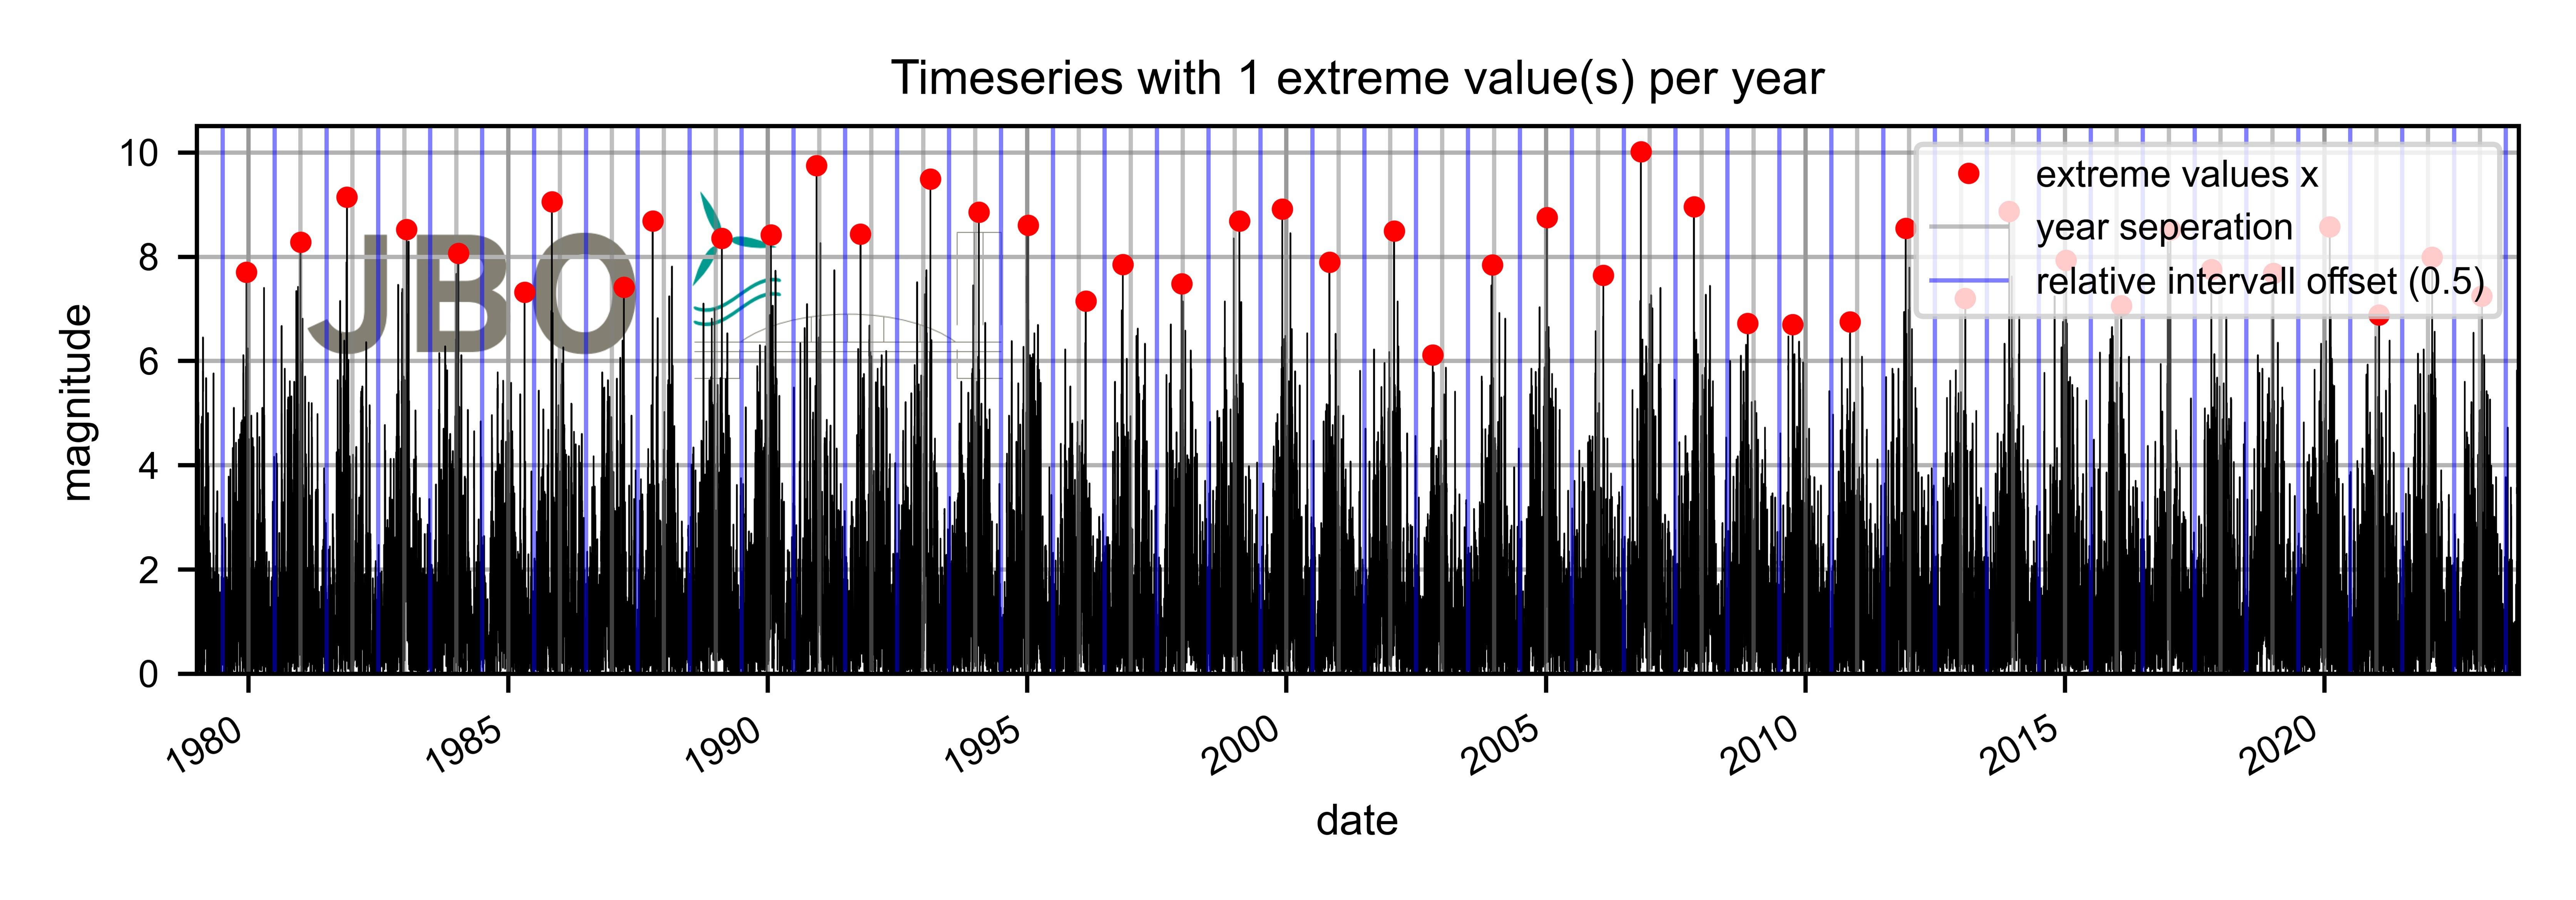
\includegraphics[width=1.0\textwidth]{C:/Users/aaron.lange/Desktop/Projekte/Hindcast_Tool/HindTool/latex_templates/Extreme_Timeseries_Example.jpg} 
 \caption{ Exemplary time series indicating extreme values on yearly separation } 
 \label{fig: Extreme_Timeseries_Example } 
\end{figure}

The Gumbel distribution considering is applied to the data set $x$ as follows:


\begin{align}
\label{eq:gumbel}
P_{G u m b}=\exp \left(-\exp \left(-\frac{x-\mu} {\beta}\right)\right) \\
\text{with: }
&\beta=\sigma \frac{\sqrt{6}}{\pi} \quad \text{(scale parameter)}\\
&\mu=\bar{x}-\gamma \beta \quad \text{(location parameter)}
\end{align}


where the standard deviation is denoted as $\sigma$, the mean value as $\bar{x}$ and the Euler-Mascheroni constant $\gamma \approx 0.5772$ . The theoretical probability $P_{t h}$ is calculated as the quantile of each of the $N$ (sorted) datapoints, following the Gumbel distribution, by using the formula:

\begin{align}
    P_{t h}=\frac{n-0.5}{N}, n=1 \ldots N
\end{align}


by finding the inverse of formula \ref{eq:gumbel}.

\begin{align}
    \label{eq:gumbel_inv}
    x_{t h}=-\beta \ln \left(-\ln P_{t h}\right)+\mu
\end{align}


Here, $n$ theoretical extreme values $x_{t h}$ are found and compared to the real extreme values $x$.

\begin{figure}[H] 
 \centering 
 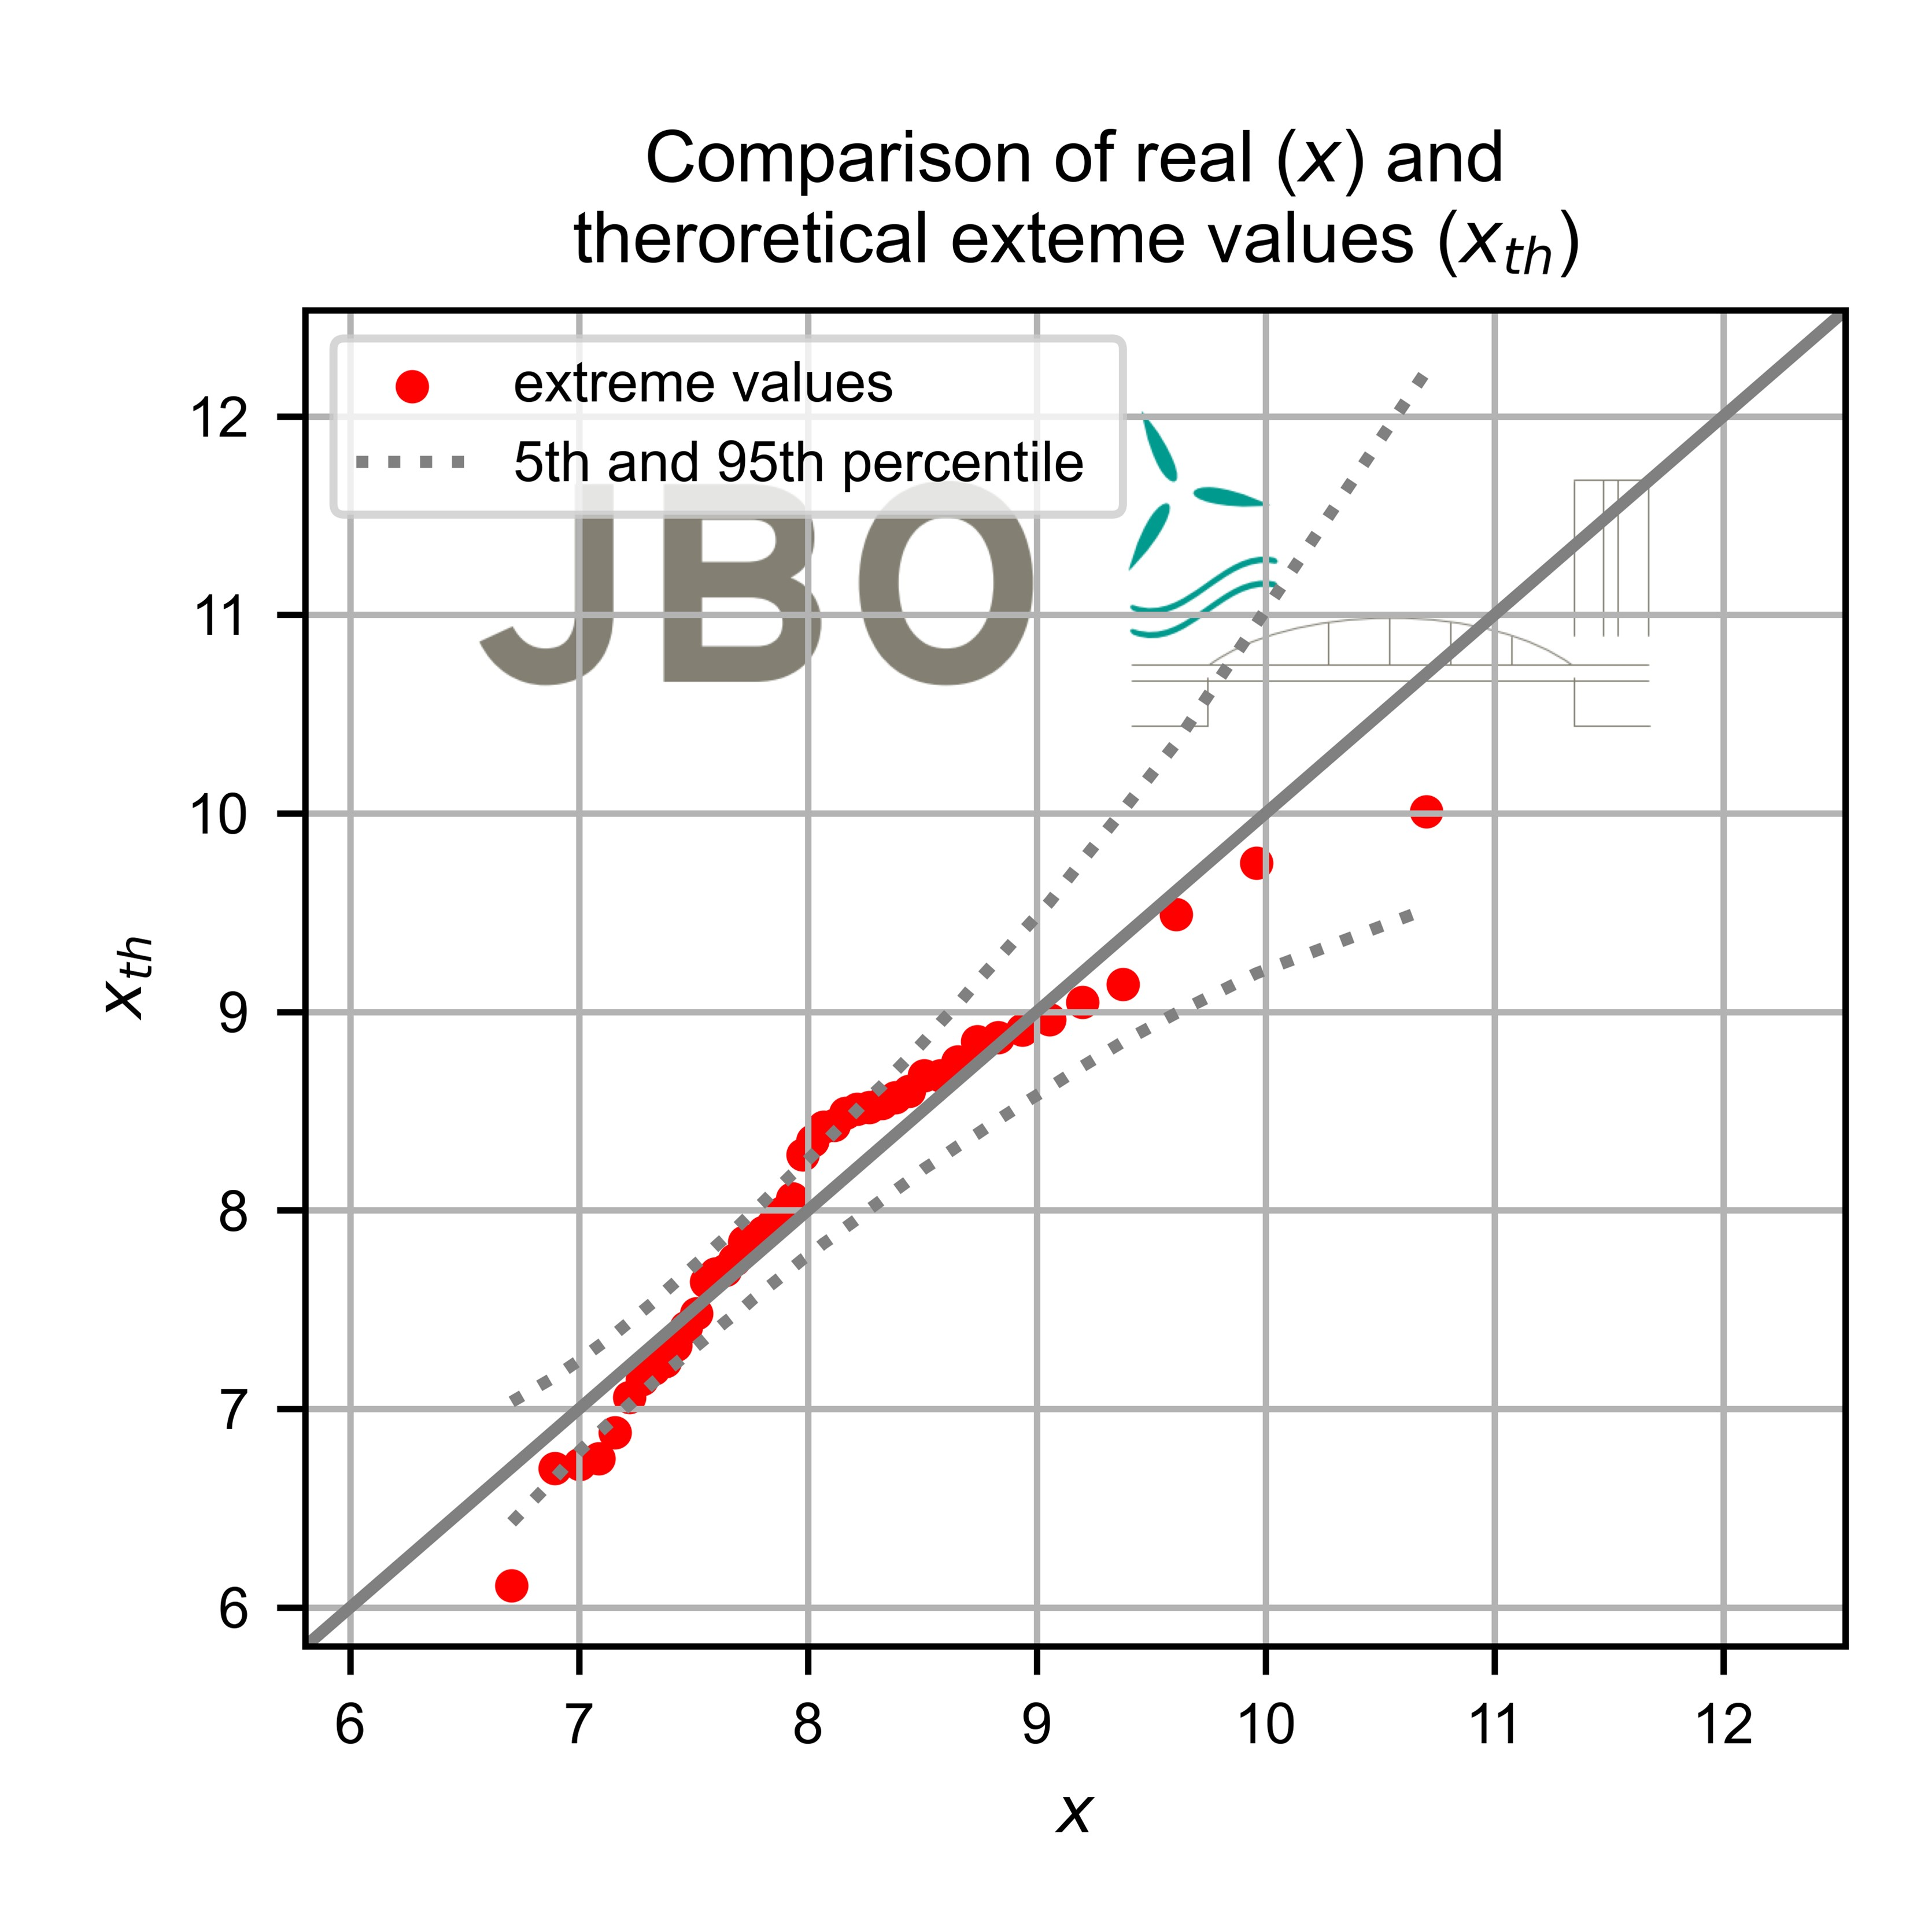
\includegraphics[width=0.5\textwidth]{C:/Users/aaron.lange/Desktop/Projekte/Hindcast_Tool/HindTool/latex_templates/Extreme_qq_example.jpg} 
 \caption{ Comparison of real and theoretical extreme values } 
 \label{fig: Extreme_qq_example } 
\end{figure}

By visually evaluating the distance from a perfect correlation, shown as the line $x=x_{t h}$, the fit of the distribution can be evaluated. Also shown are the percentiles of the Gumbel distribution. These are numerically determined. $N$ uniformly distributed probabilities $p_{n} \in[0,1], n=1 \ldots N$ are generated and the corresponding theoretical extreme values are found using equation \ref{eq:gumbel}. This is repeated many times ( $N_{\text {rep }}$ ) and each of the resulting sets of size $N$ are sorted by magnitude. Now for each magnitude rank with size $N_{\text {rep }}$ any percentile can be calculated and is associated with the theoretical extreme values $x_{t h}$.

For finding the return periods $T_{R}$ corresponding to the probability value $P$ or vice versa, the formulas below can be applied (see $[\mathrm{N} 1]$ ).

\begin{align}
\label{eq:P_to_TR}
   P=\left(1-\frac{1}{n T_{R}}\right) \quad T_{R}=\frac{1}{(1-P) n}
\end{align}


Starting from a return period, Eq. \ref{eq:P_to_TR} can be used to the probability P. From there, the inverse Gumbel distribution (Eq. \ref{eq:gumbel_inv}) can be used to determine the expected extreme value. Therefore, a logarithmic grid of return periods in the required range $T_{R, j}, j=1 \ldots M$ is created and the corresponding theoretical extreme values $x_{j, m i d}$ are determined.

For finding the confidence intervals, labelled $x_{j, \sigma}$ and $x_{j,-\sigma}$, another numerical method is applied. For each of the $i$ determined sets $p_{n}$, new Gumbel coefficients $\beta_{i}$ and $\sigma_{i}$ are calculated. For each of the return periods $T_{R, j}$, the corresponding probabilities $P_{j}$ of the current Gumbel distribution are found. The result is a $N_{r e p}$ by $M$ matrix, in which there are a big number ( $N_{r e p}$ ) of extreme values corresponding to the return periods $T_{R, j}$ on the logarithmic grid. Those can be used to determine the standard deviation $\sigma_{j}$ for each of the $j$ return periods $T_{R, j}$. As suggested in REF, these values can be simply added or subtracted to the appropriate value $x_{j, m i d}$ :

$$
\begin{aligned}
x_{j,+\sigma}=x_{j, \text{mid}}+\sigma_{j} \\
x_{j,-\sigma}=x_{j, \text{mid}}-\sigma_{j}
\end{aligned}
$$

Furthermore, the expected magnitudes and confidence intervals for any needed return periods can be determined by interpolating the found correlations.\\


\begin{figure}[H] 
 \centering 
 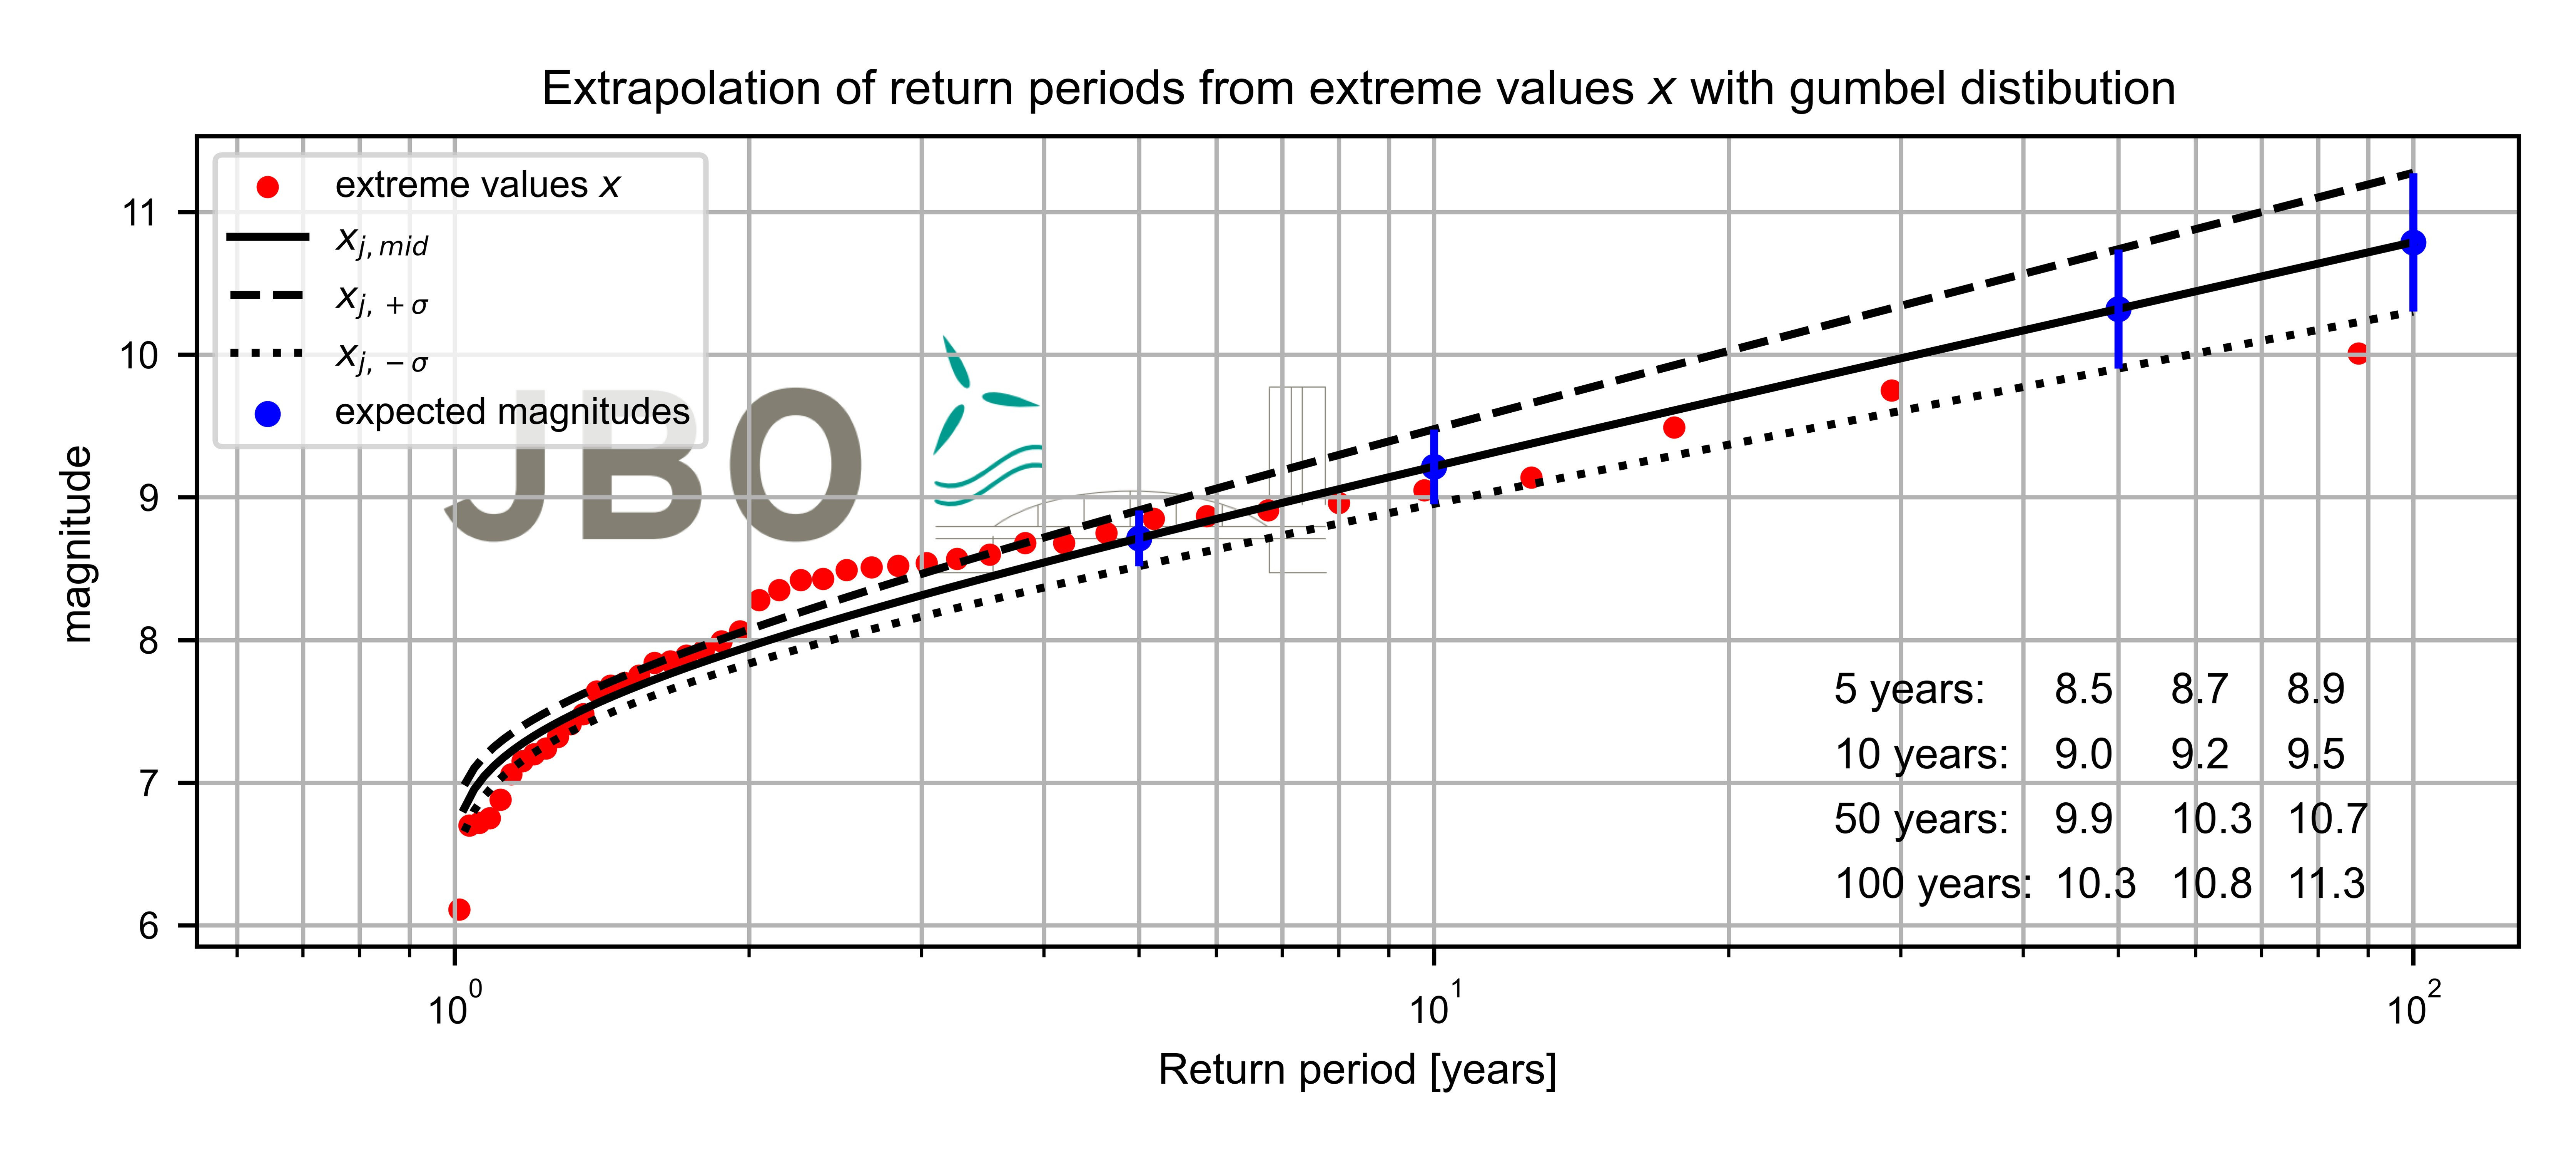
\includegraphics[width=1.0\textwidth]{C:/Users/aaron.lange/Desktop/Projekte/Hindcast_Tool/HindTool/latex_templates/Extreme_TReturn_example.jpg} 
 \caption{ Extrapolation of return periods with standard deviation } 
 \label{fig: Extreme_TReturn_example } 
\end{figure}

\clearpage


\subsubsection{Data Evaluation: Maximal Wave Height [m]} 
\begin{figure}[H] 
 \centering 
 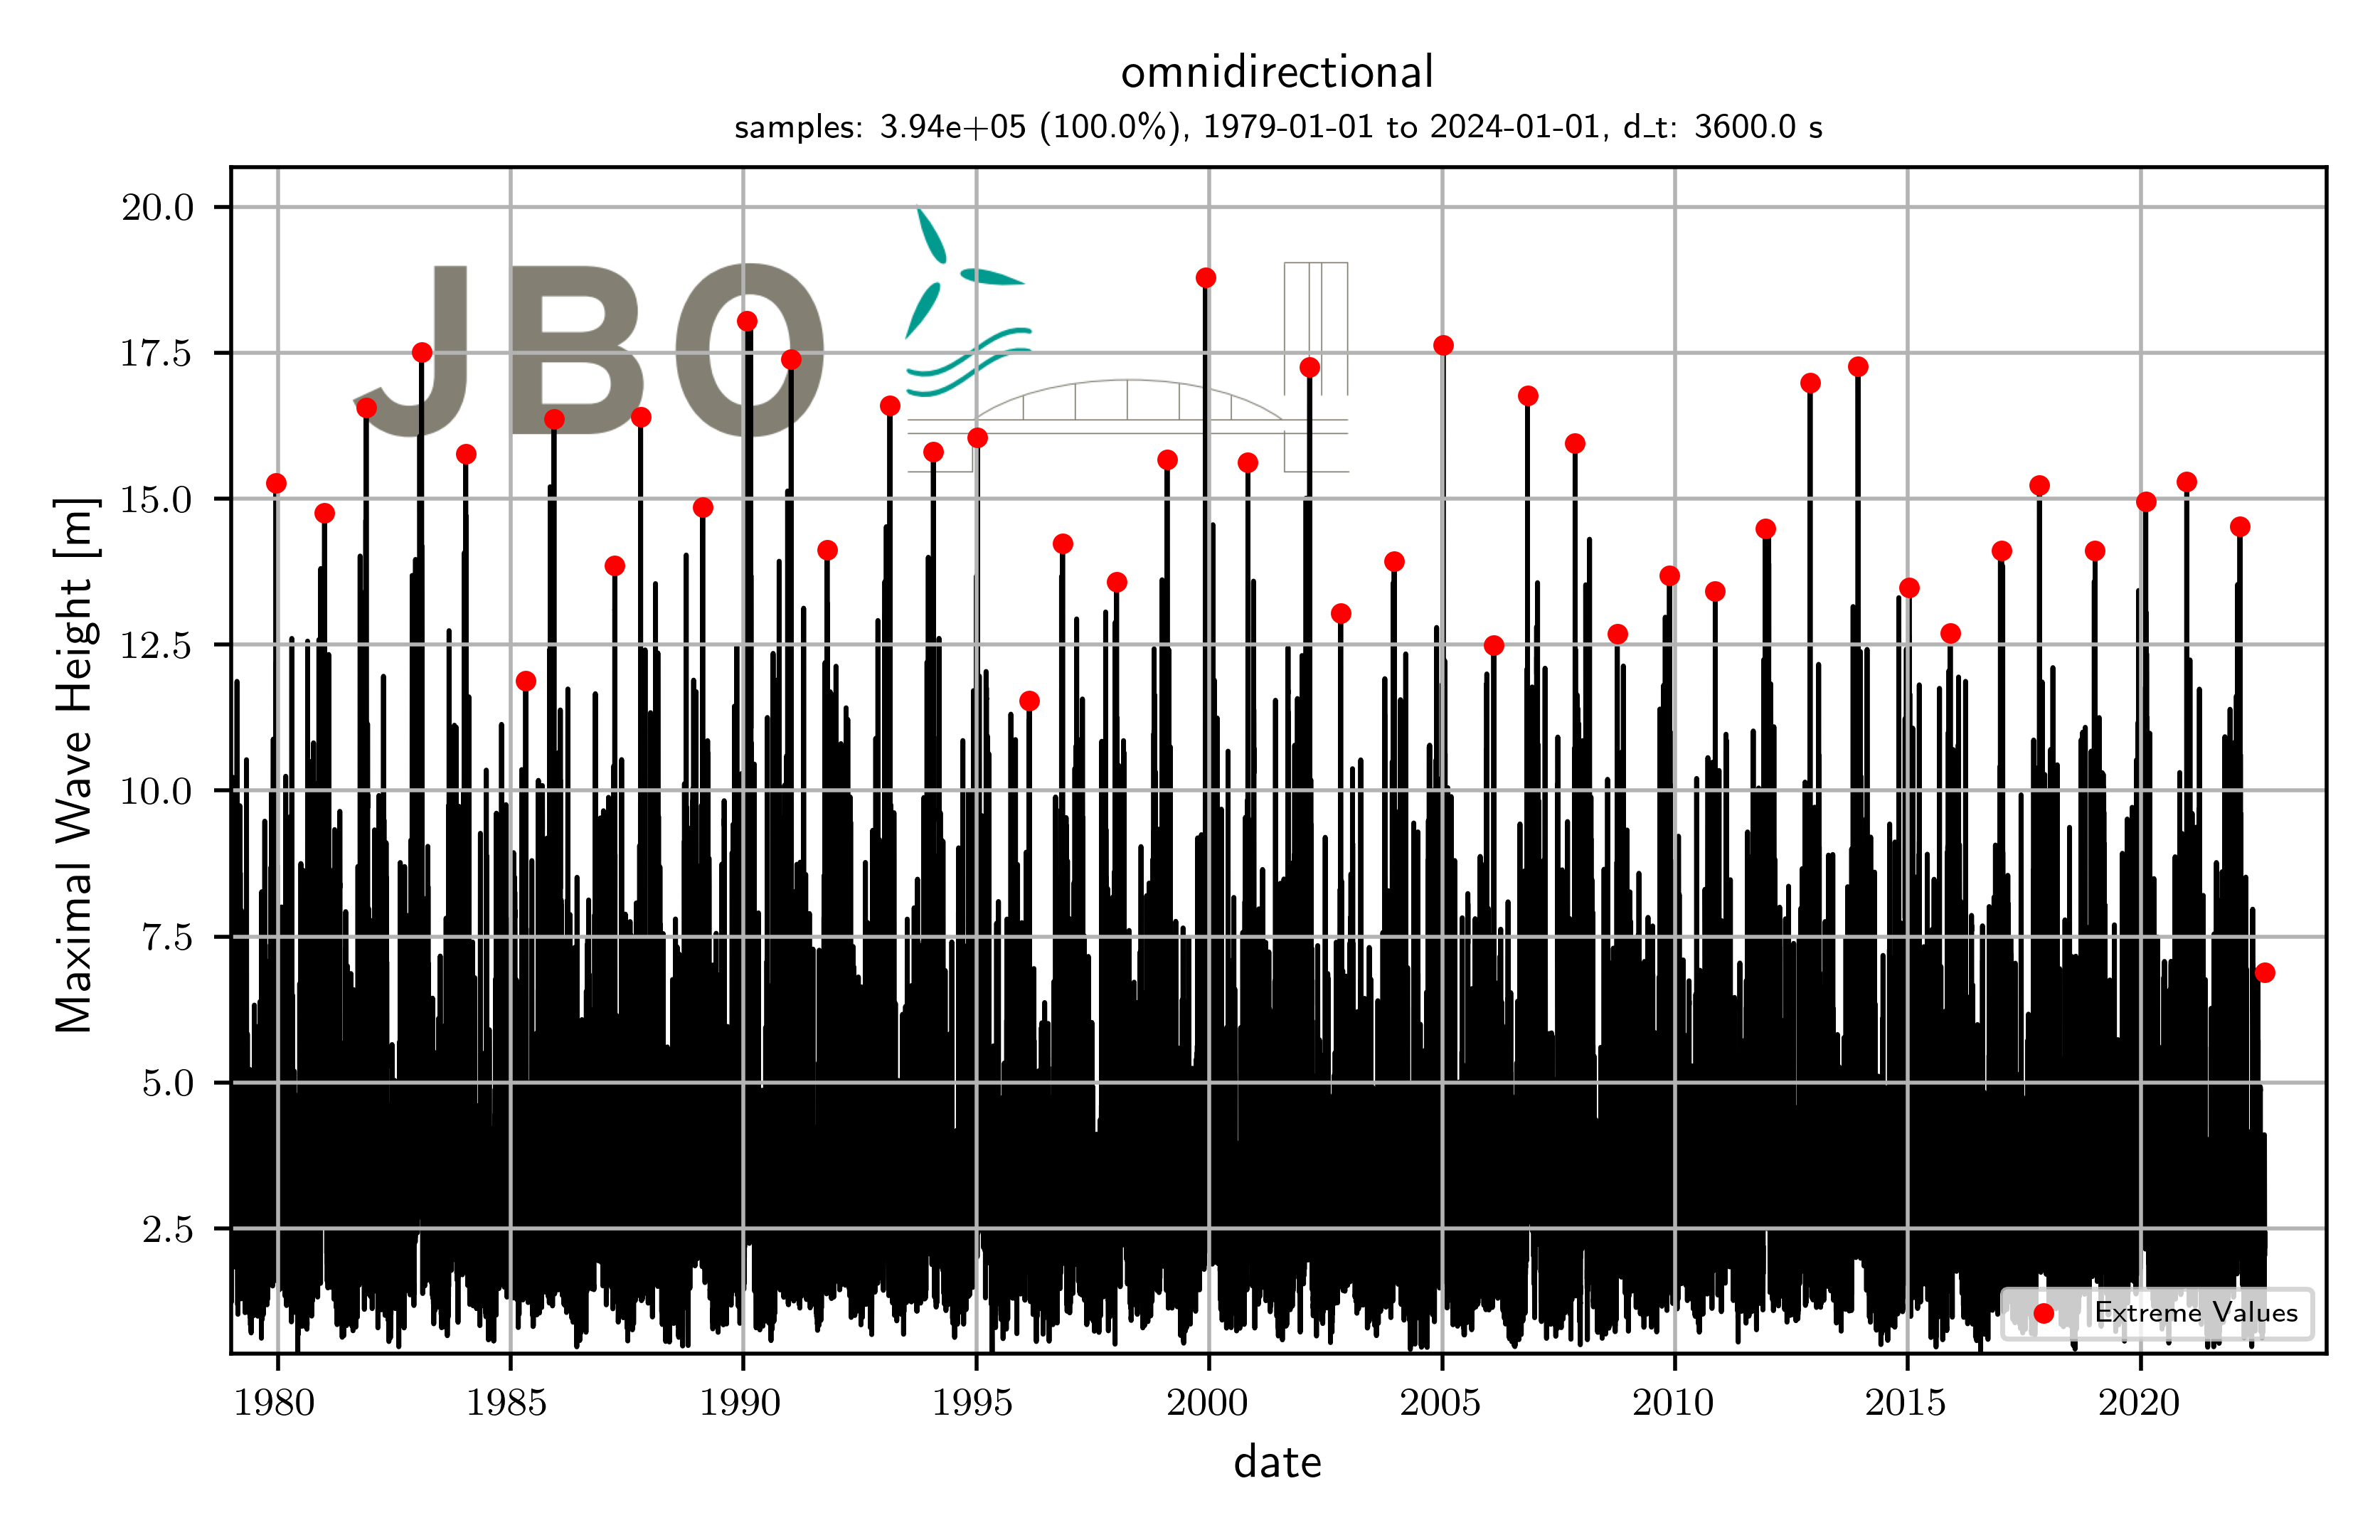
\includegraphics[width=1.0\textwidth]{C:/Users/aaron.lange/Desktop/Projekte/Hindcast_Tool/HindTool/example_output/Extreme_Timeseries_WaveHeight_page_3.png} 
 \caption{ Extreme-Timeseries-WaveHeight-page-3 } 
 \label{fig: Extreme_Timeseries_WaveHeight_page_3 } 
\end{figure}
\begin{figure}[H] 
 \centering 
 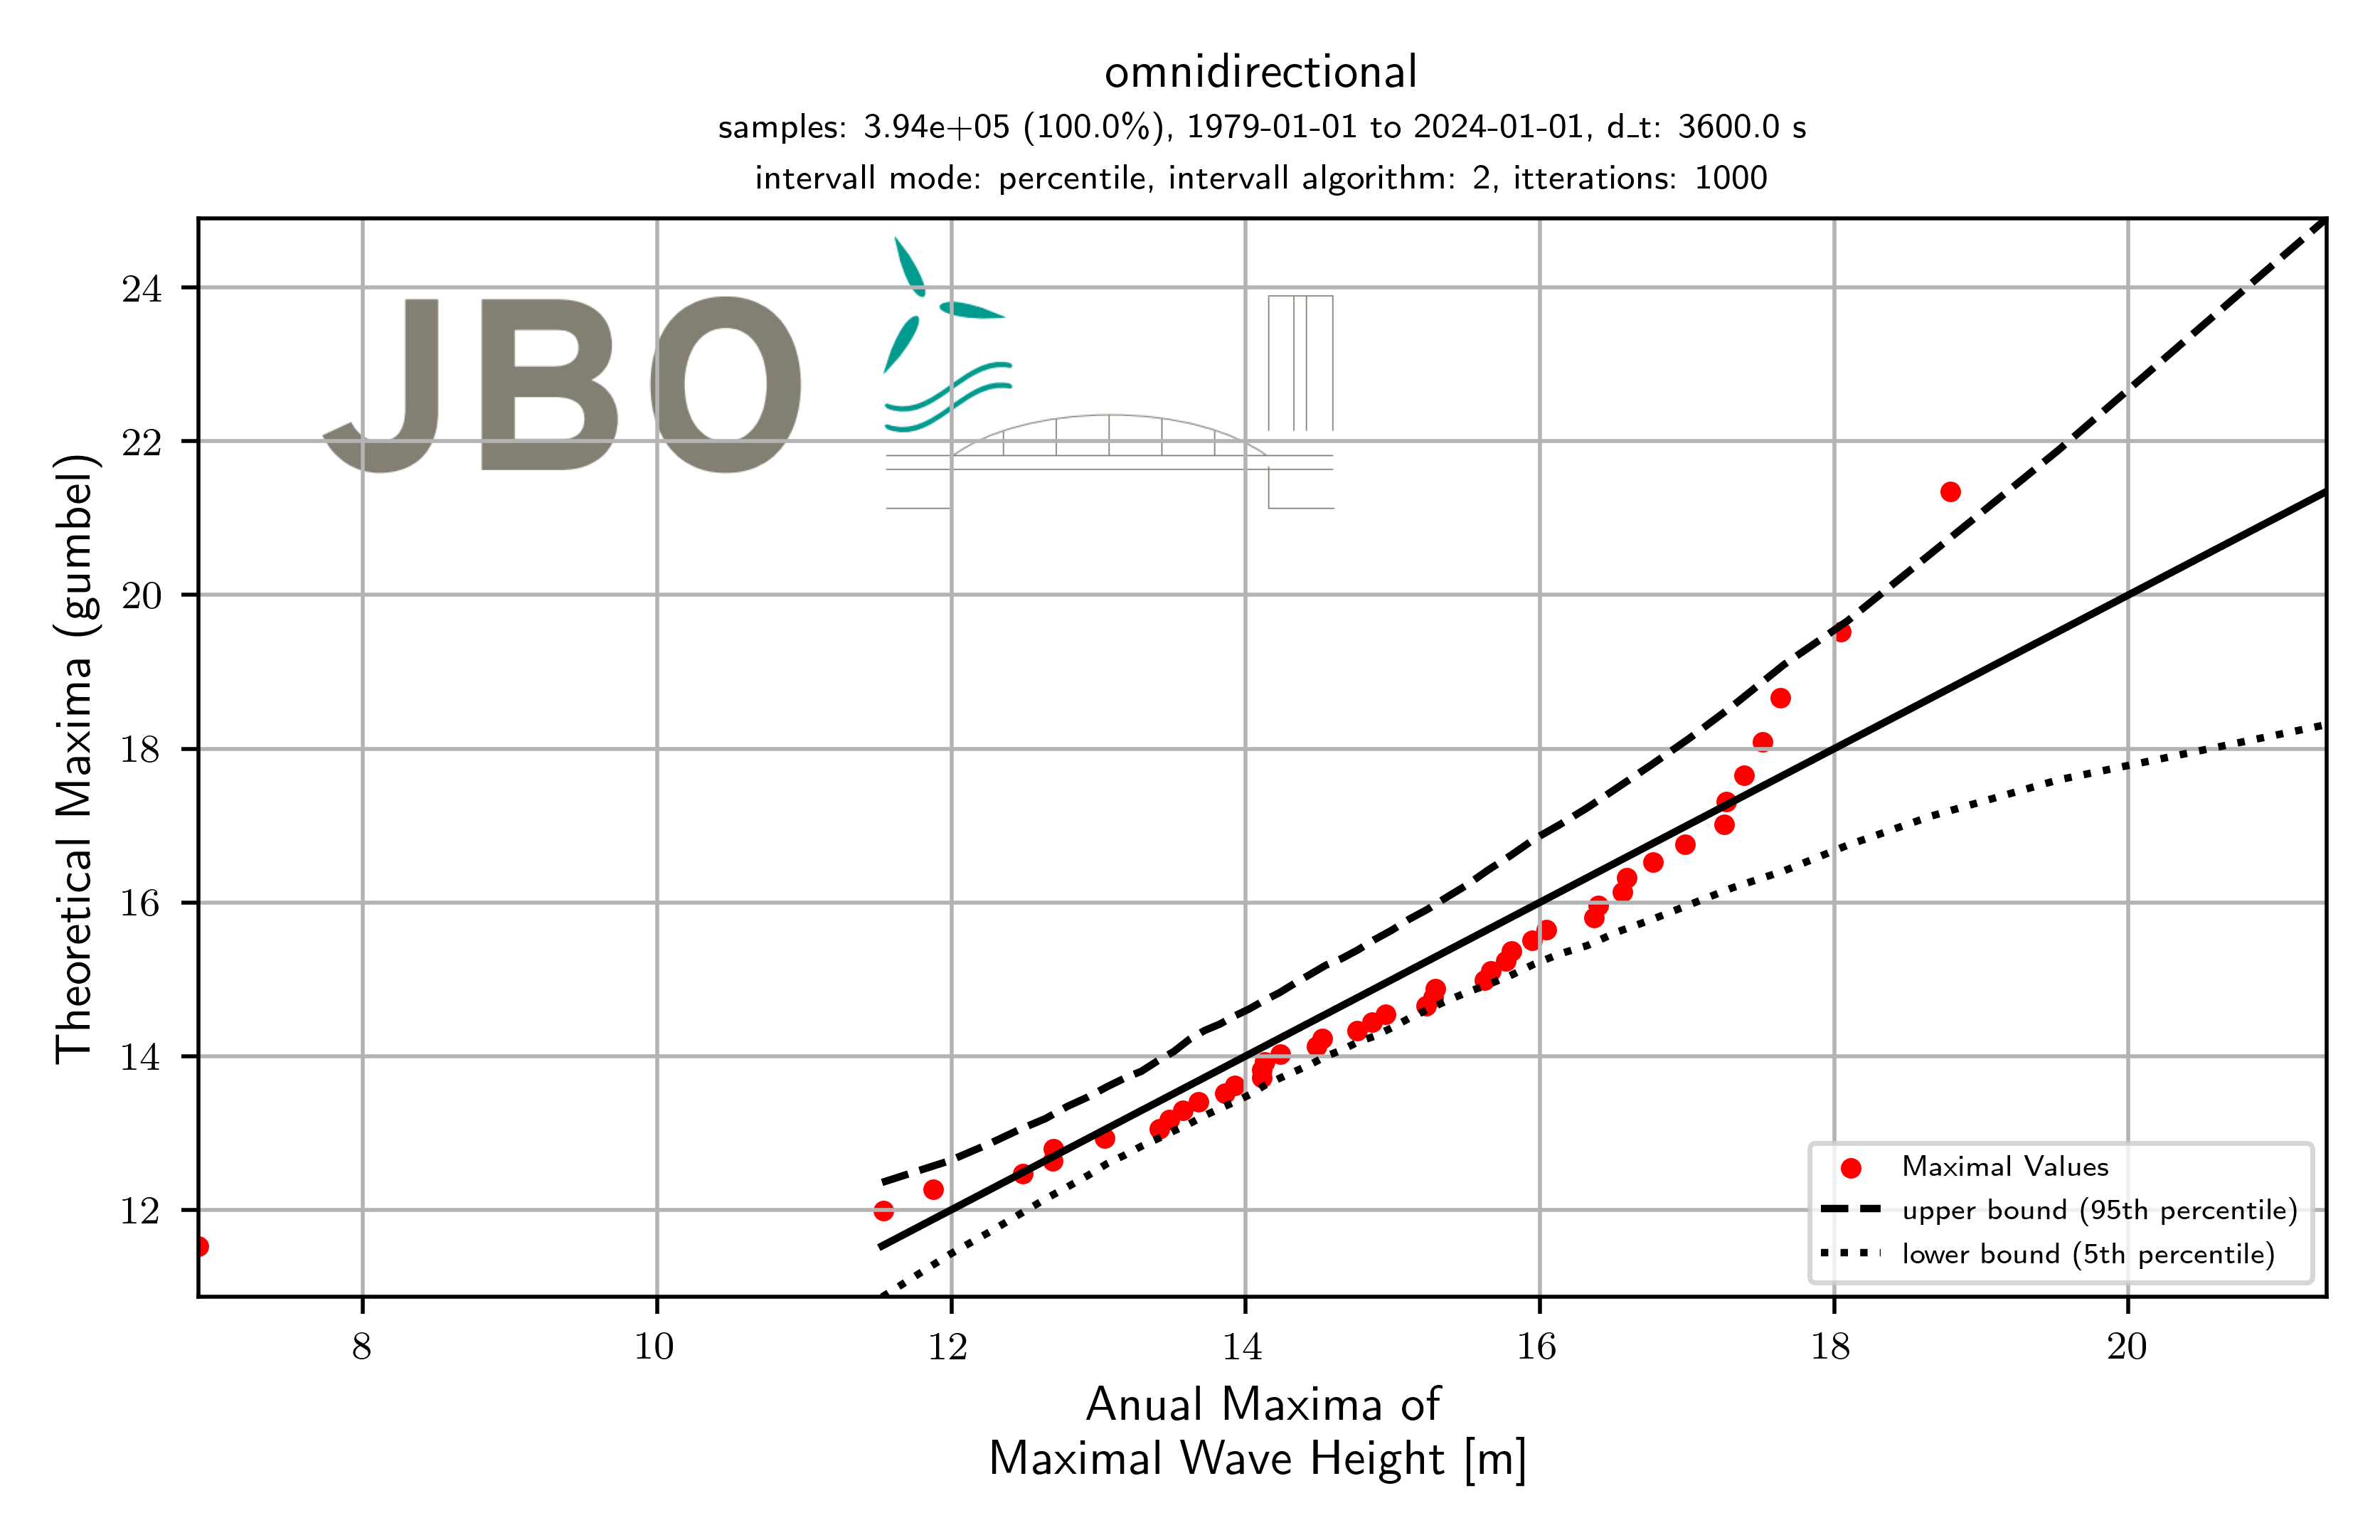
\includegraphics[width=1.0\textwidth]{C:/Users/aaron.lange/Desktop/Projekte/Hindcast_Tool/HindTool/example_output/Extreme_qq_WaveHeight_page_3.png} 
 \caption{ Extreme-qq-WaveHeight-page-3 } 
 \label{fig: Extreme_qq_WaveHeight_page_3 } 
\end{figure}
\begin{figure}[H] 
 \centering 
 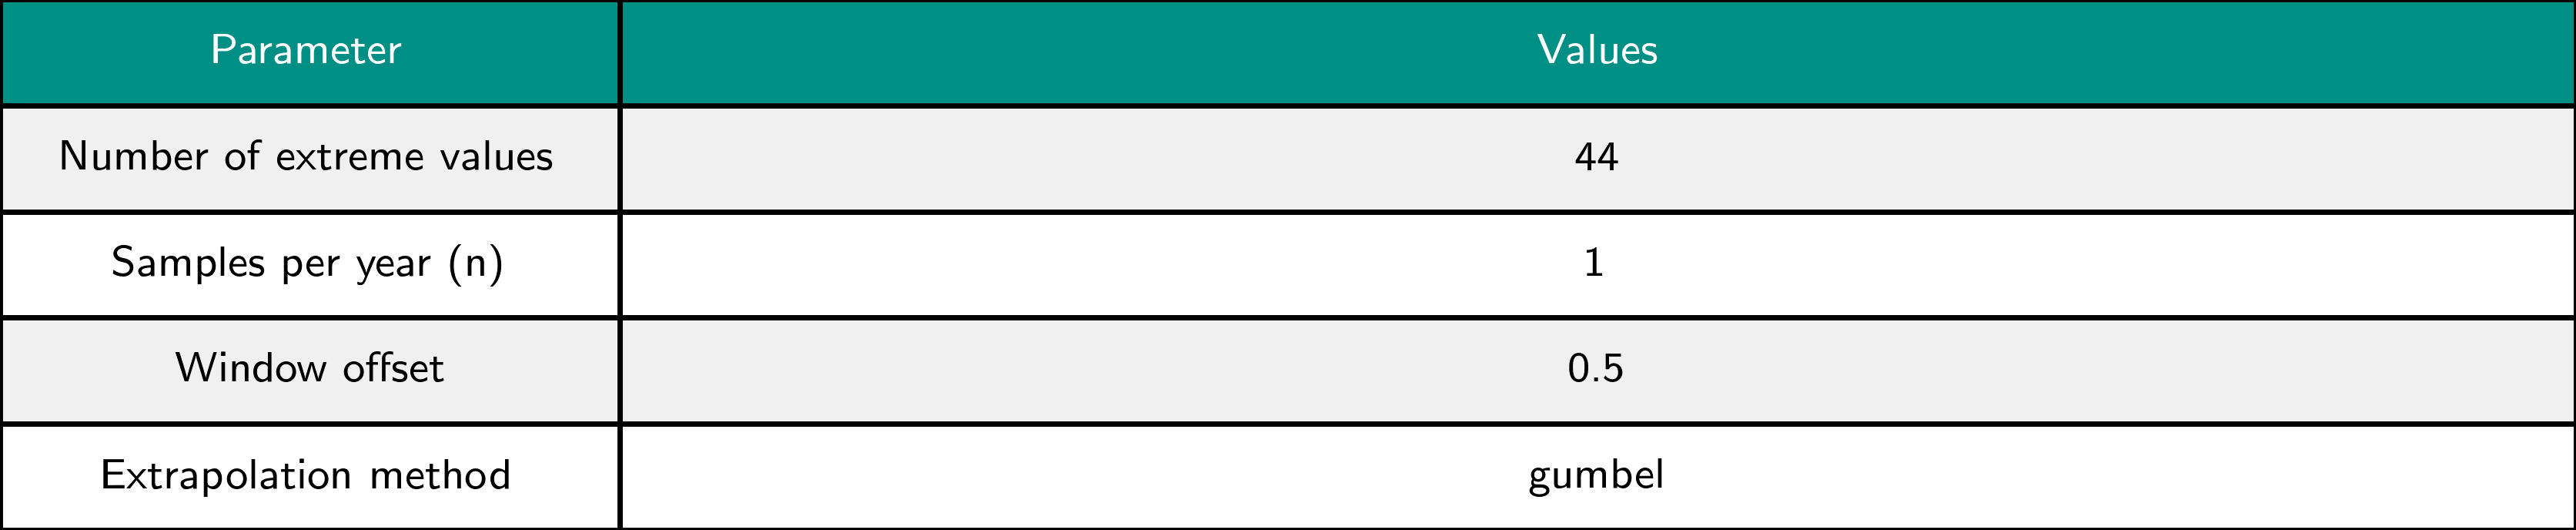
\includegraphics[width=1.0\textwidth ]{C:/Users/aaron.lange/Desktop/Projekte/Hindcast_Tool/HindTool/example_output/Extreme_Parameter_table_WaveHeight_page_1.png} 
 \captionsetup{type=table} 
\caption{ Extreme-Parameter-table-WaveHeight-page-1 } 
 \label{tab: Extreme_Parameter_table_WaveHeight_page_1 } 
\end{figure}
\begin{figure}[H] 
 \centering 
 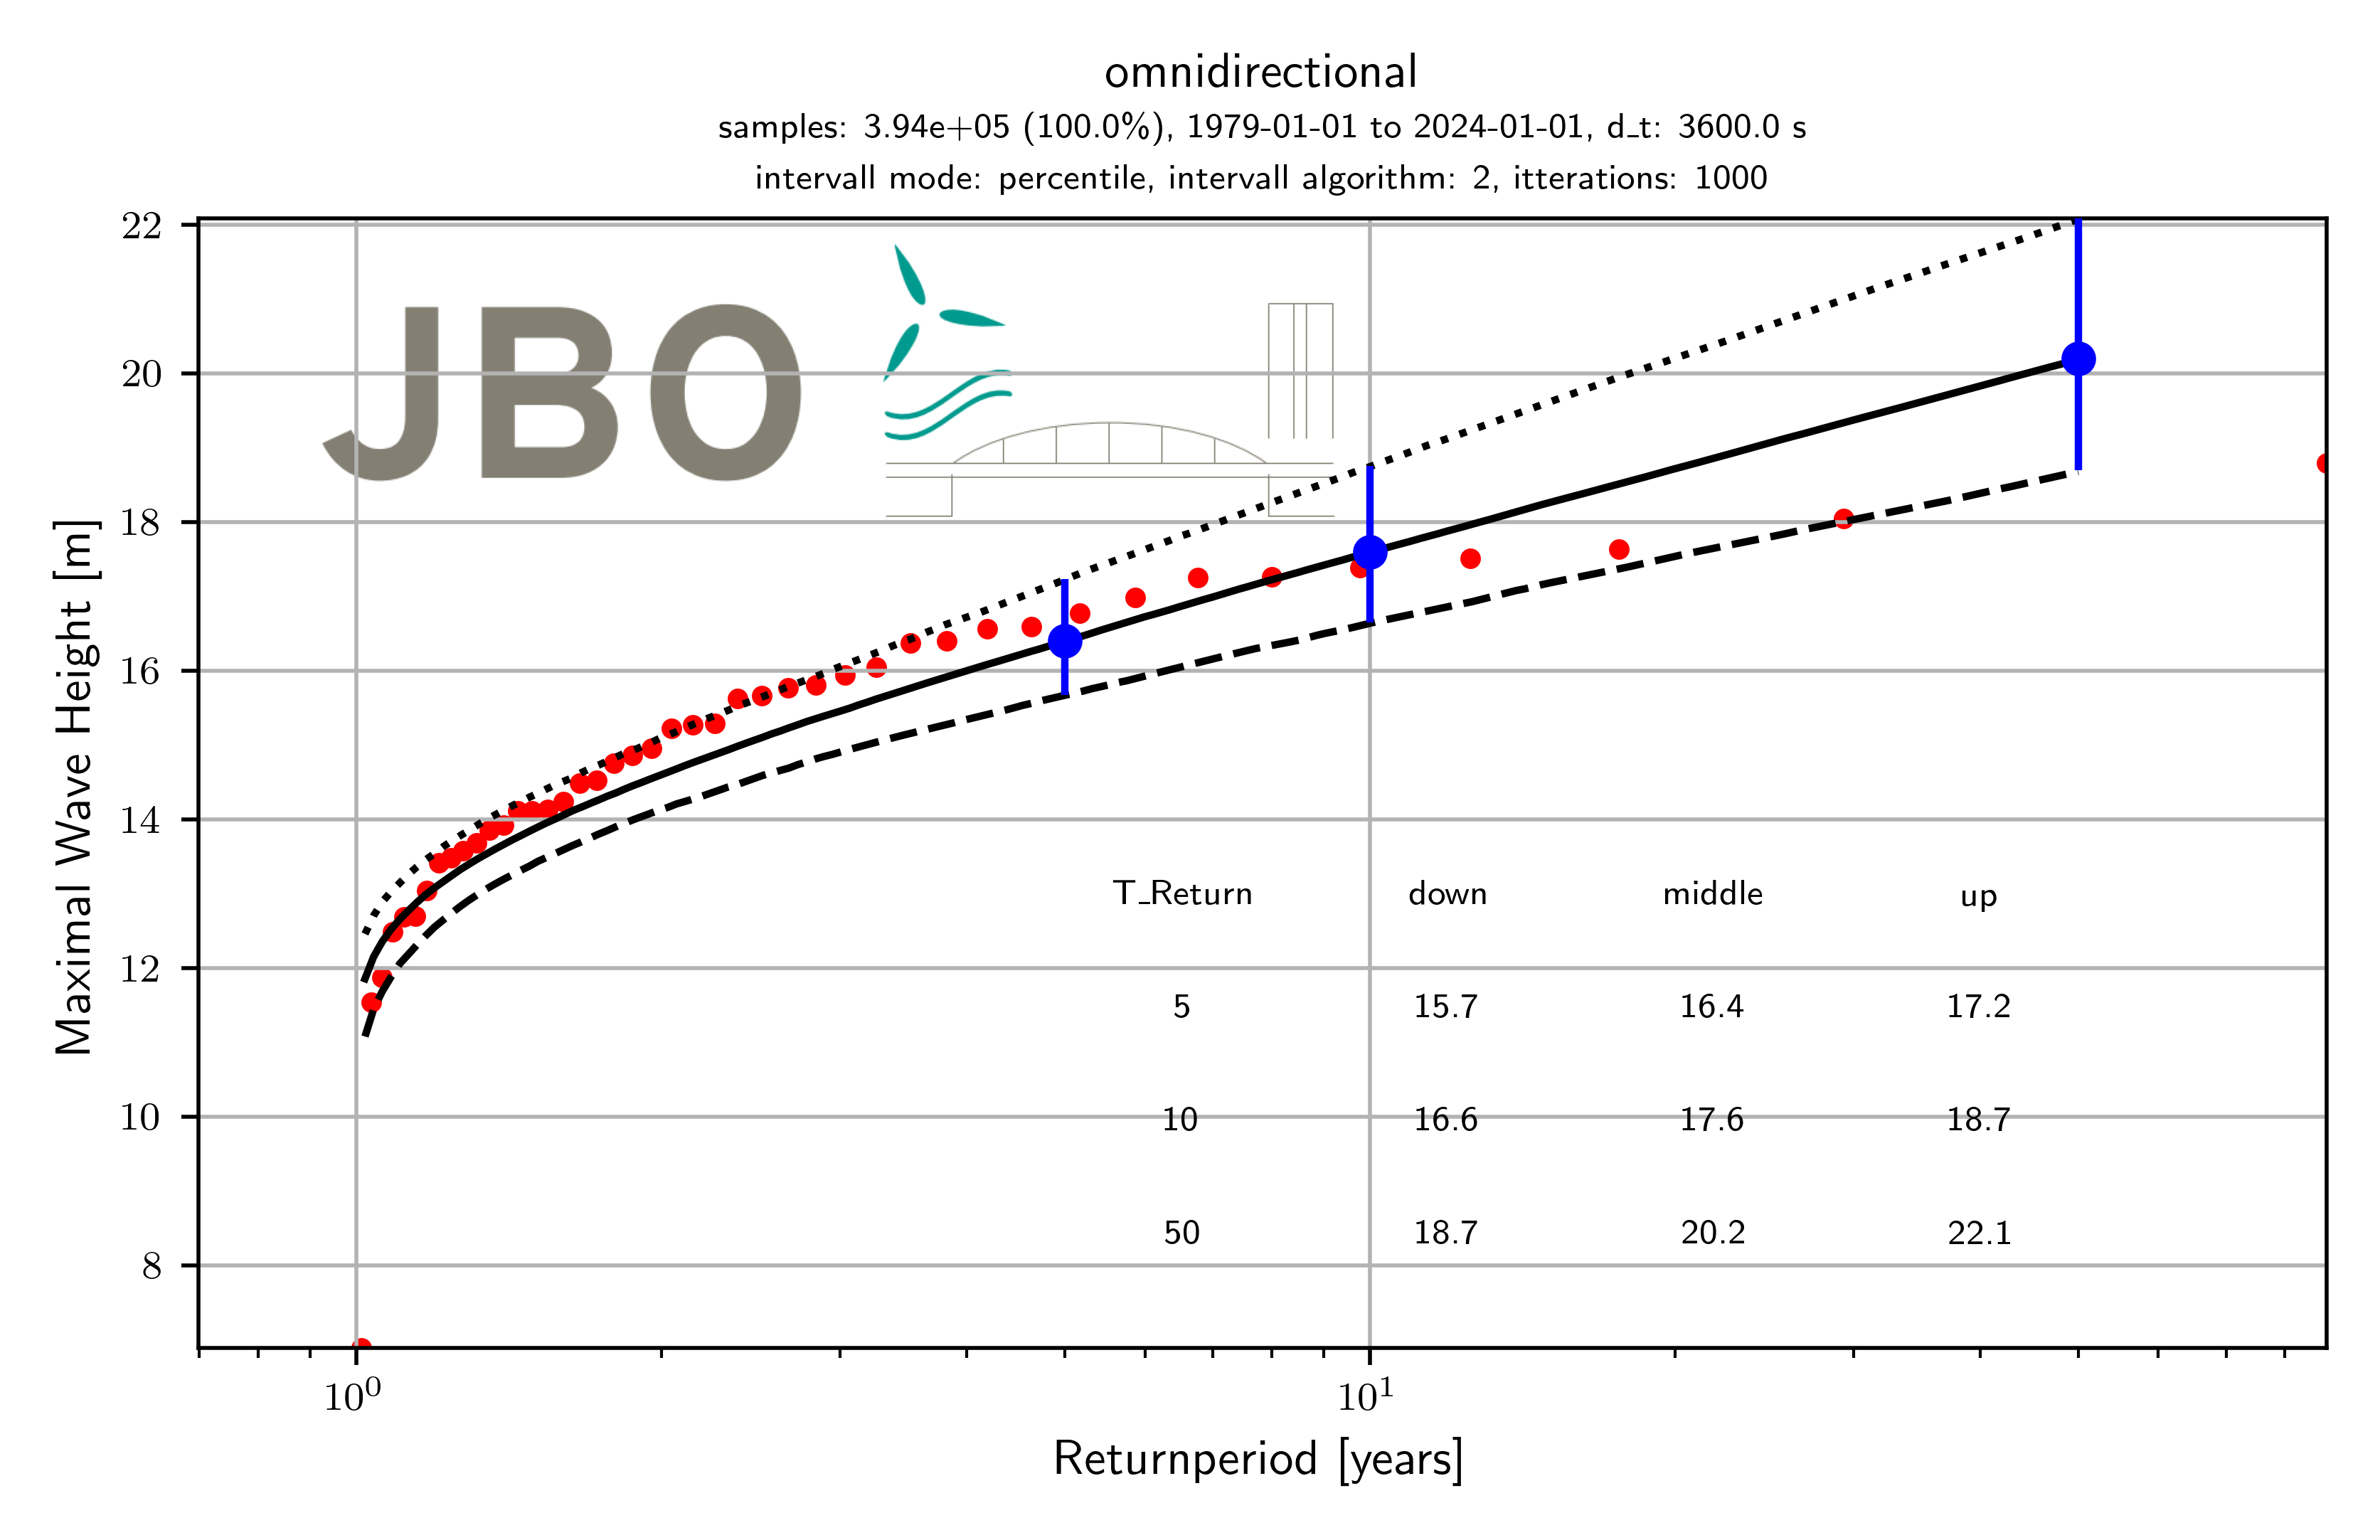
\includegraphics[width=1.0\textwidth]{C:/Users/aaron.lange/Desktop/Projekte/Hindcast_Tool/HindTool/example_output/Extreme_T_return_WaveHeight_page_3.png} 
 \caption{ Extreme-T-return-WaveHeight-page-3 } 
 \label{fig: Extreme_T_return_WaveHeight_page_3 } 
\end{figure}
\begin{figure}[H] 
 \centering 
 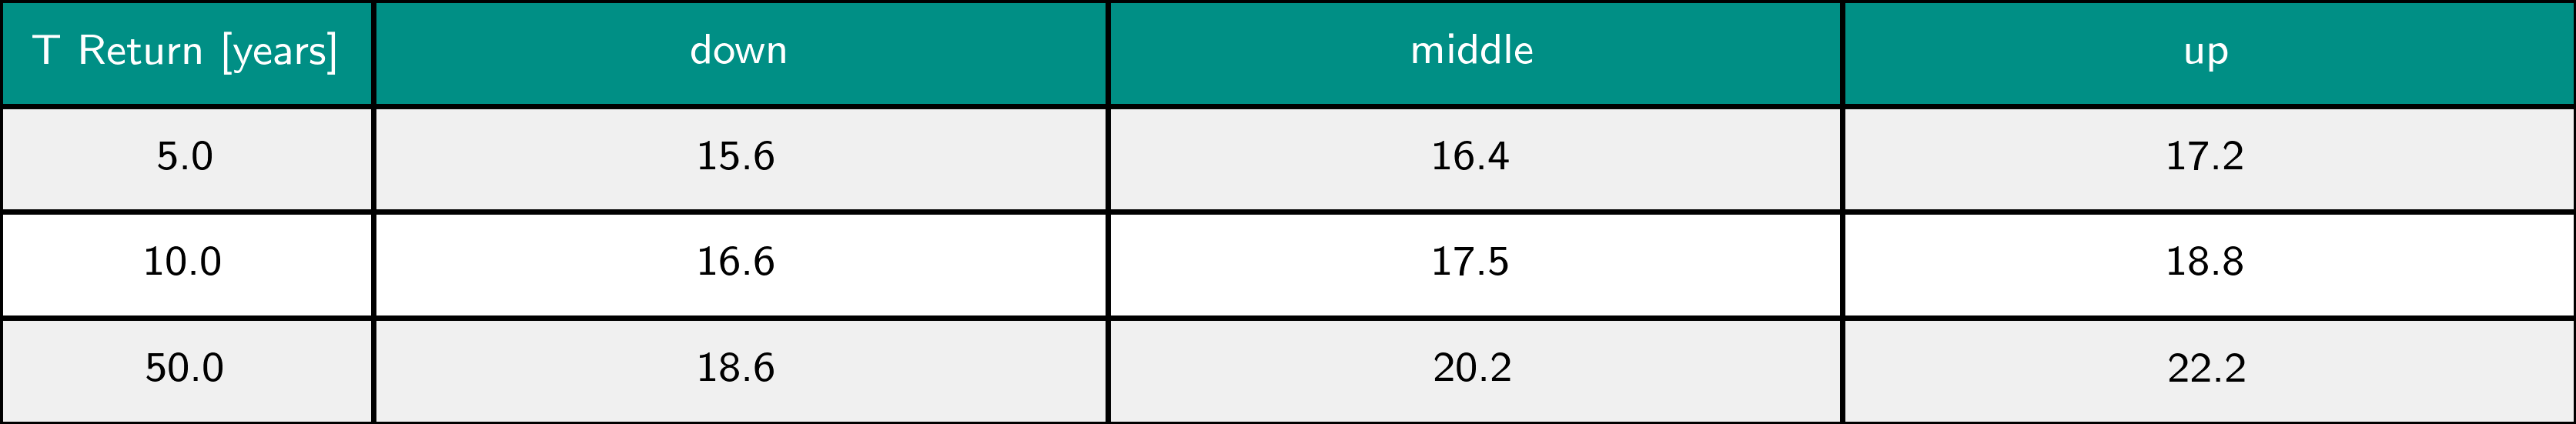
\includegraphics[width=1.0\textwidth ]{C:/Users/aaron.lange/Desktop/Projekte/Hindcast_Tool/HindTool/example_output/T_return_table_WaveHeight_page_1.png} 
 \captionsetup{type=table} 
\caption{ T-return-table-WaveHeight-page-1 } 
 \label{tab: T_return_table_WaveHeight_page_1 } 
\end{figure}
\begin{figure}[H] 
 \centering 
 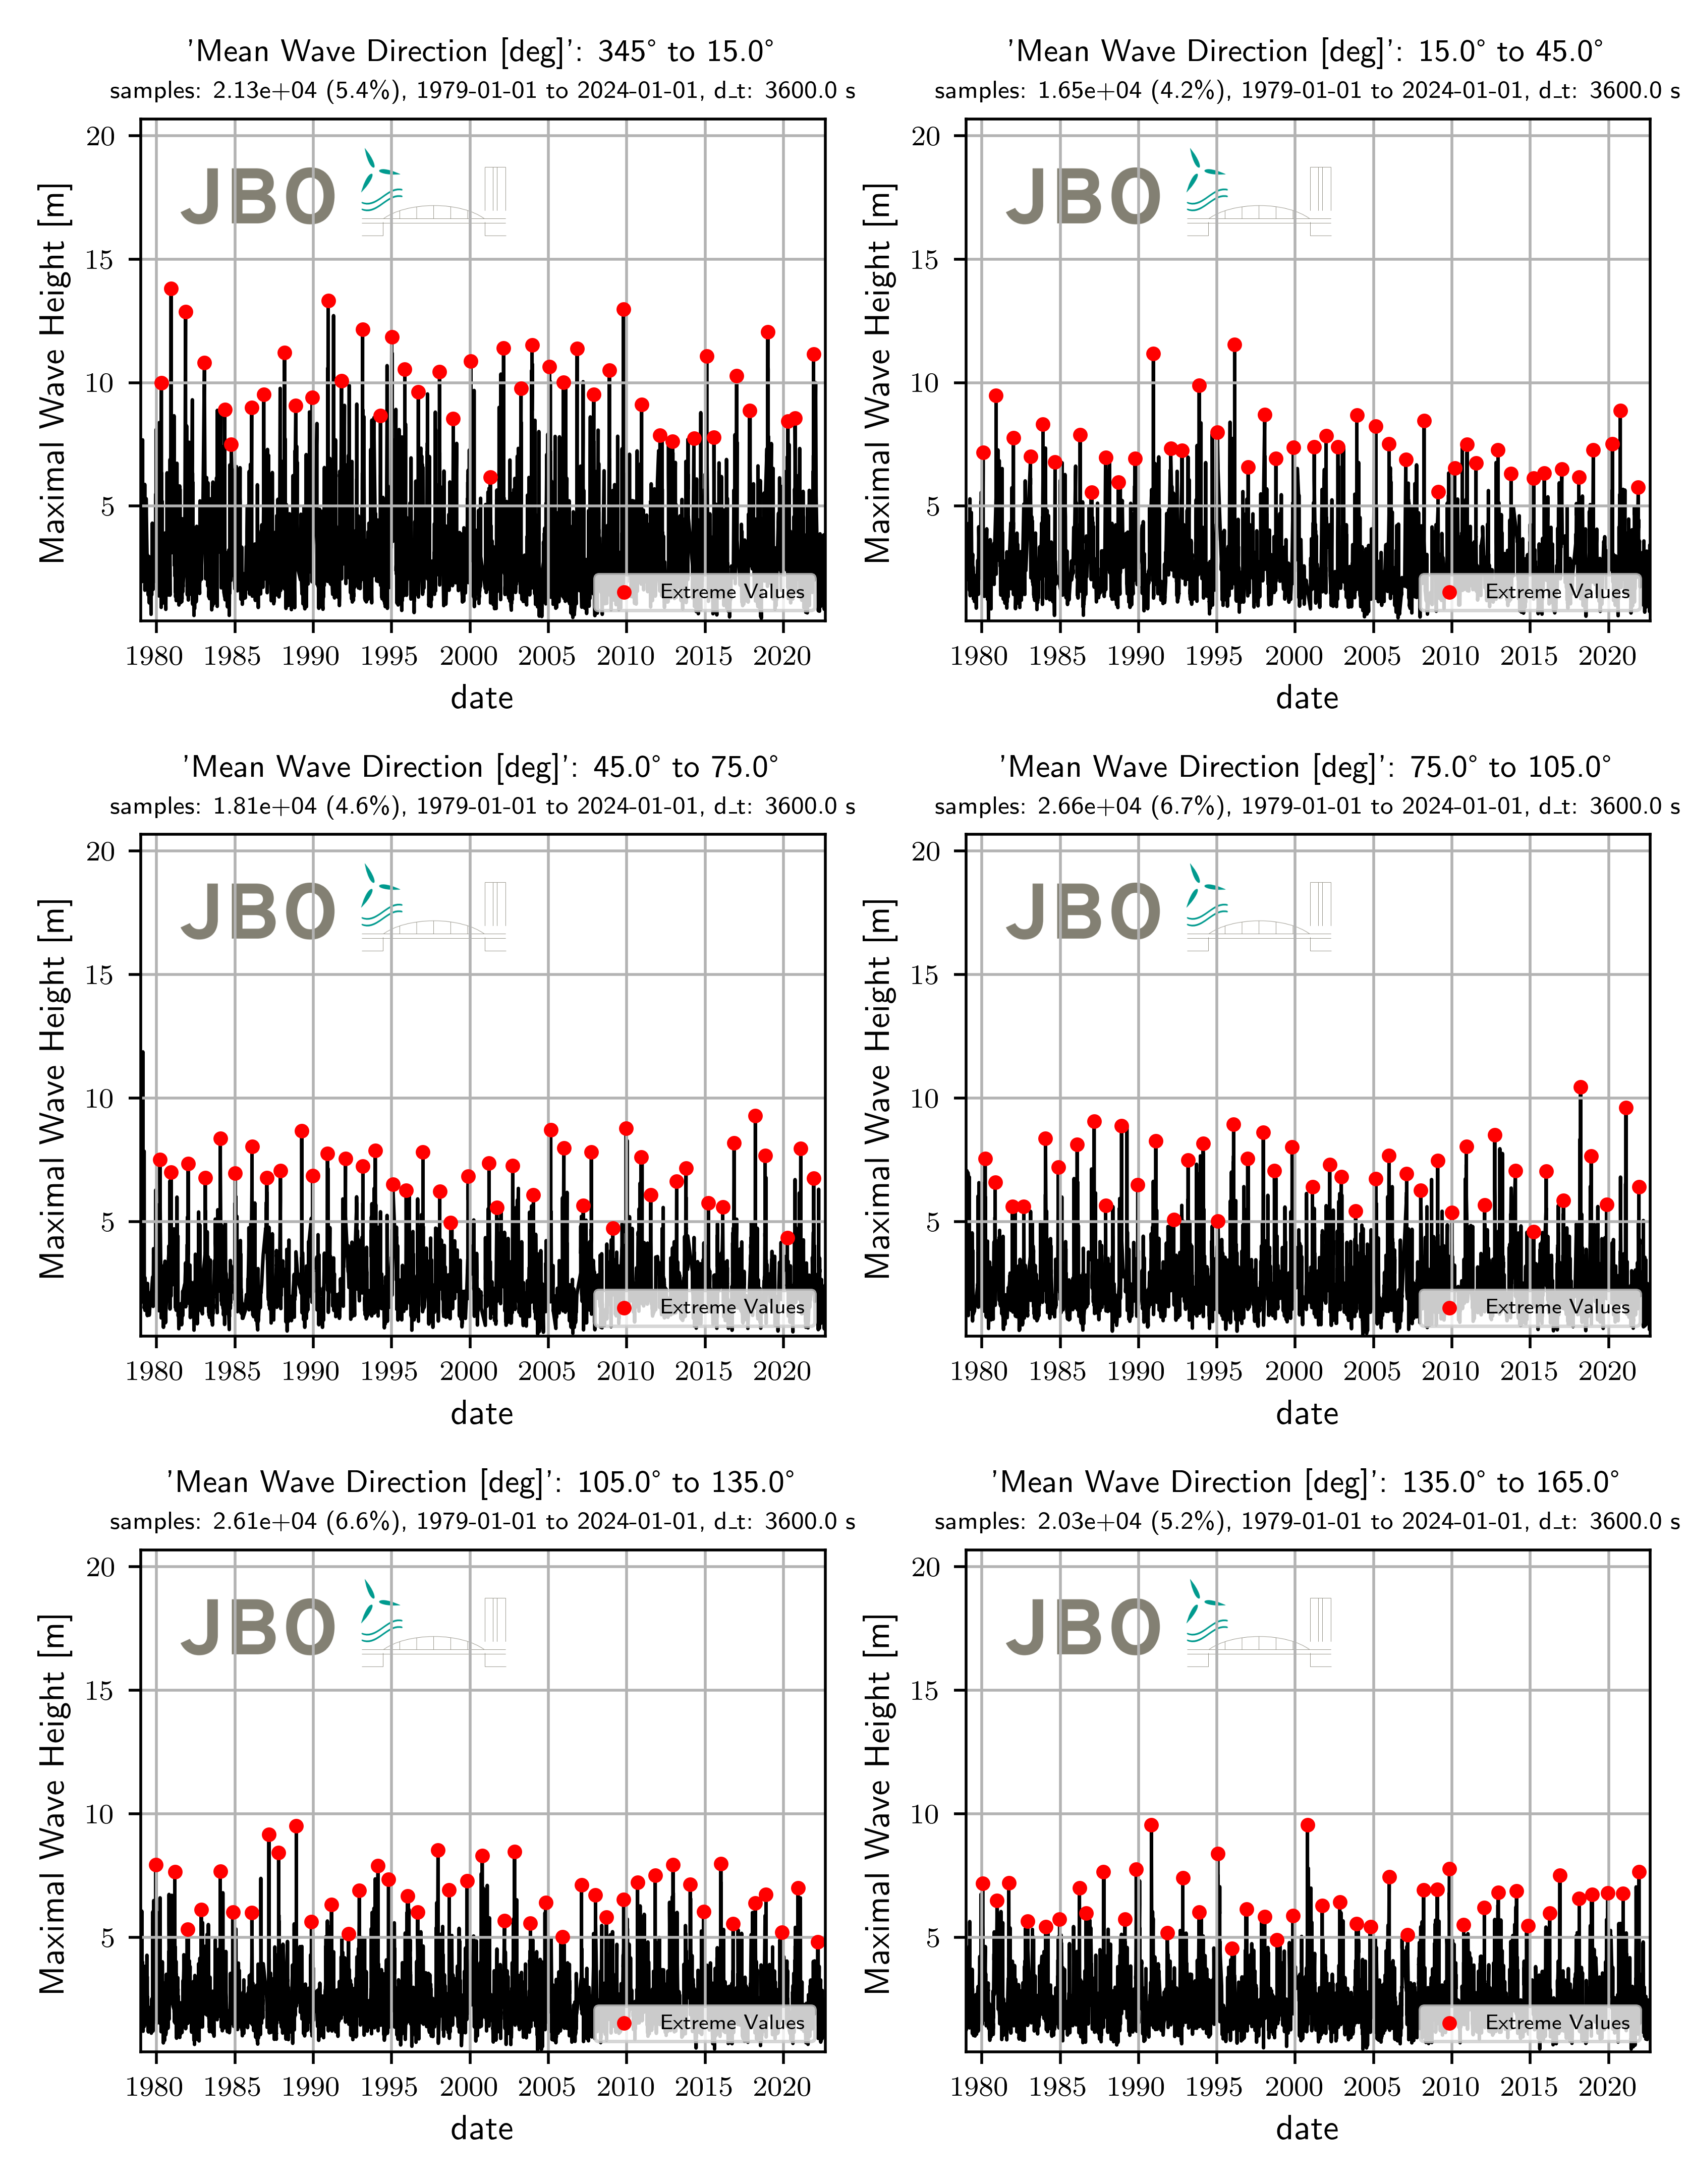
\includegraphics[width=1.0\textwidth]{C:/Users/aaron.lange/Desktop/Projekte/Hindcast_Tool/HindTool/example_output/Extreme_Timeseries_WaveHeight_page_1.png} 
 \caption{ Extreme-Timeseries-WaveHeight-page-1 } 
 \label{fig: Extreme_Timeseries_WaveHeight_page_1 } 
\end{figure}
\begin{figure}[H] 
 \centering 
 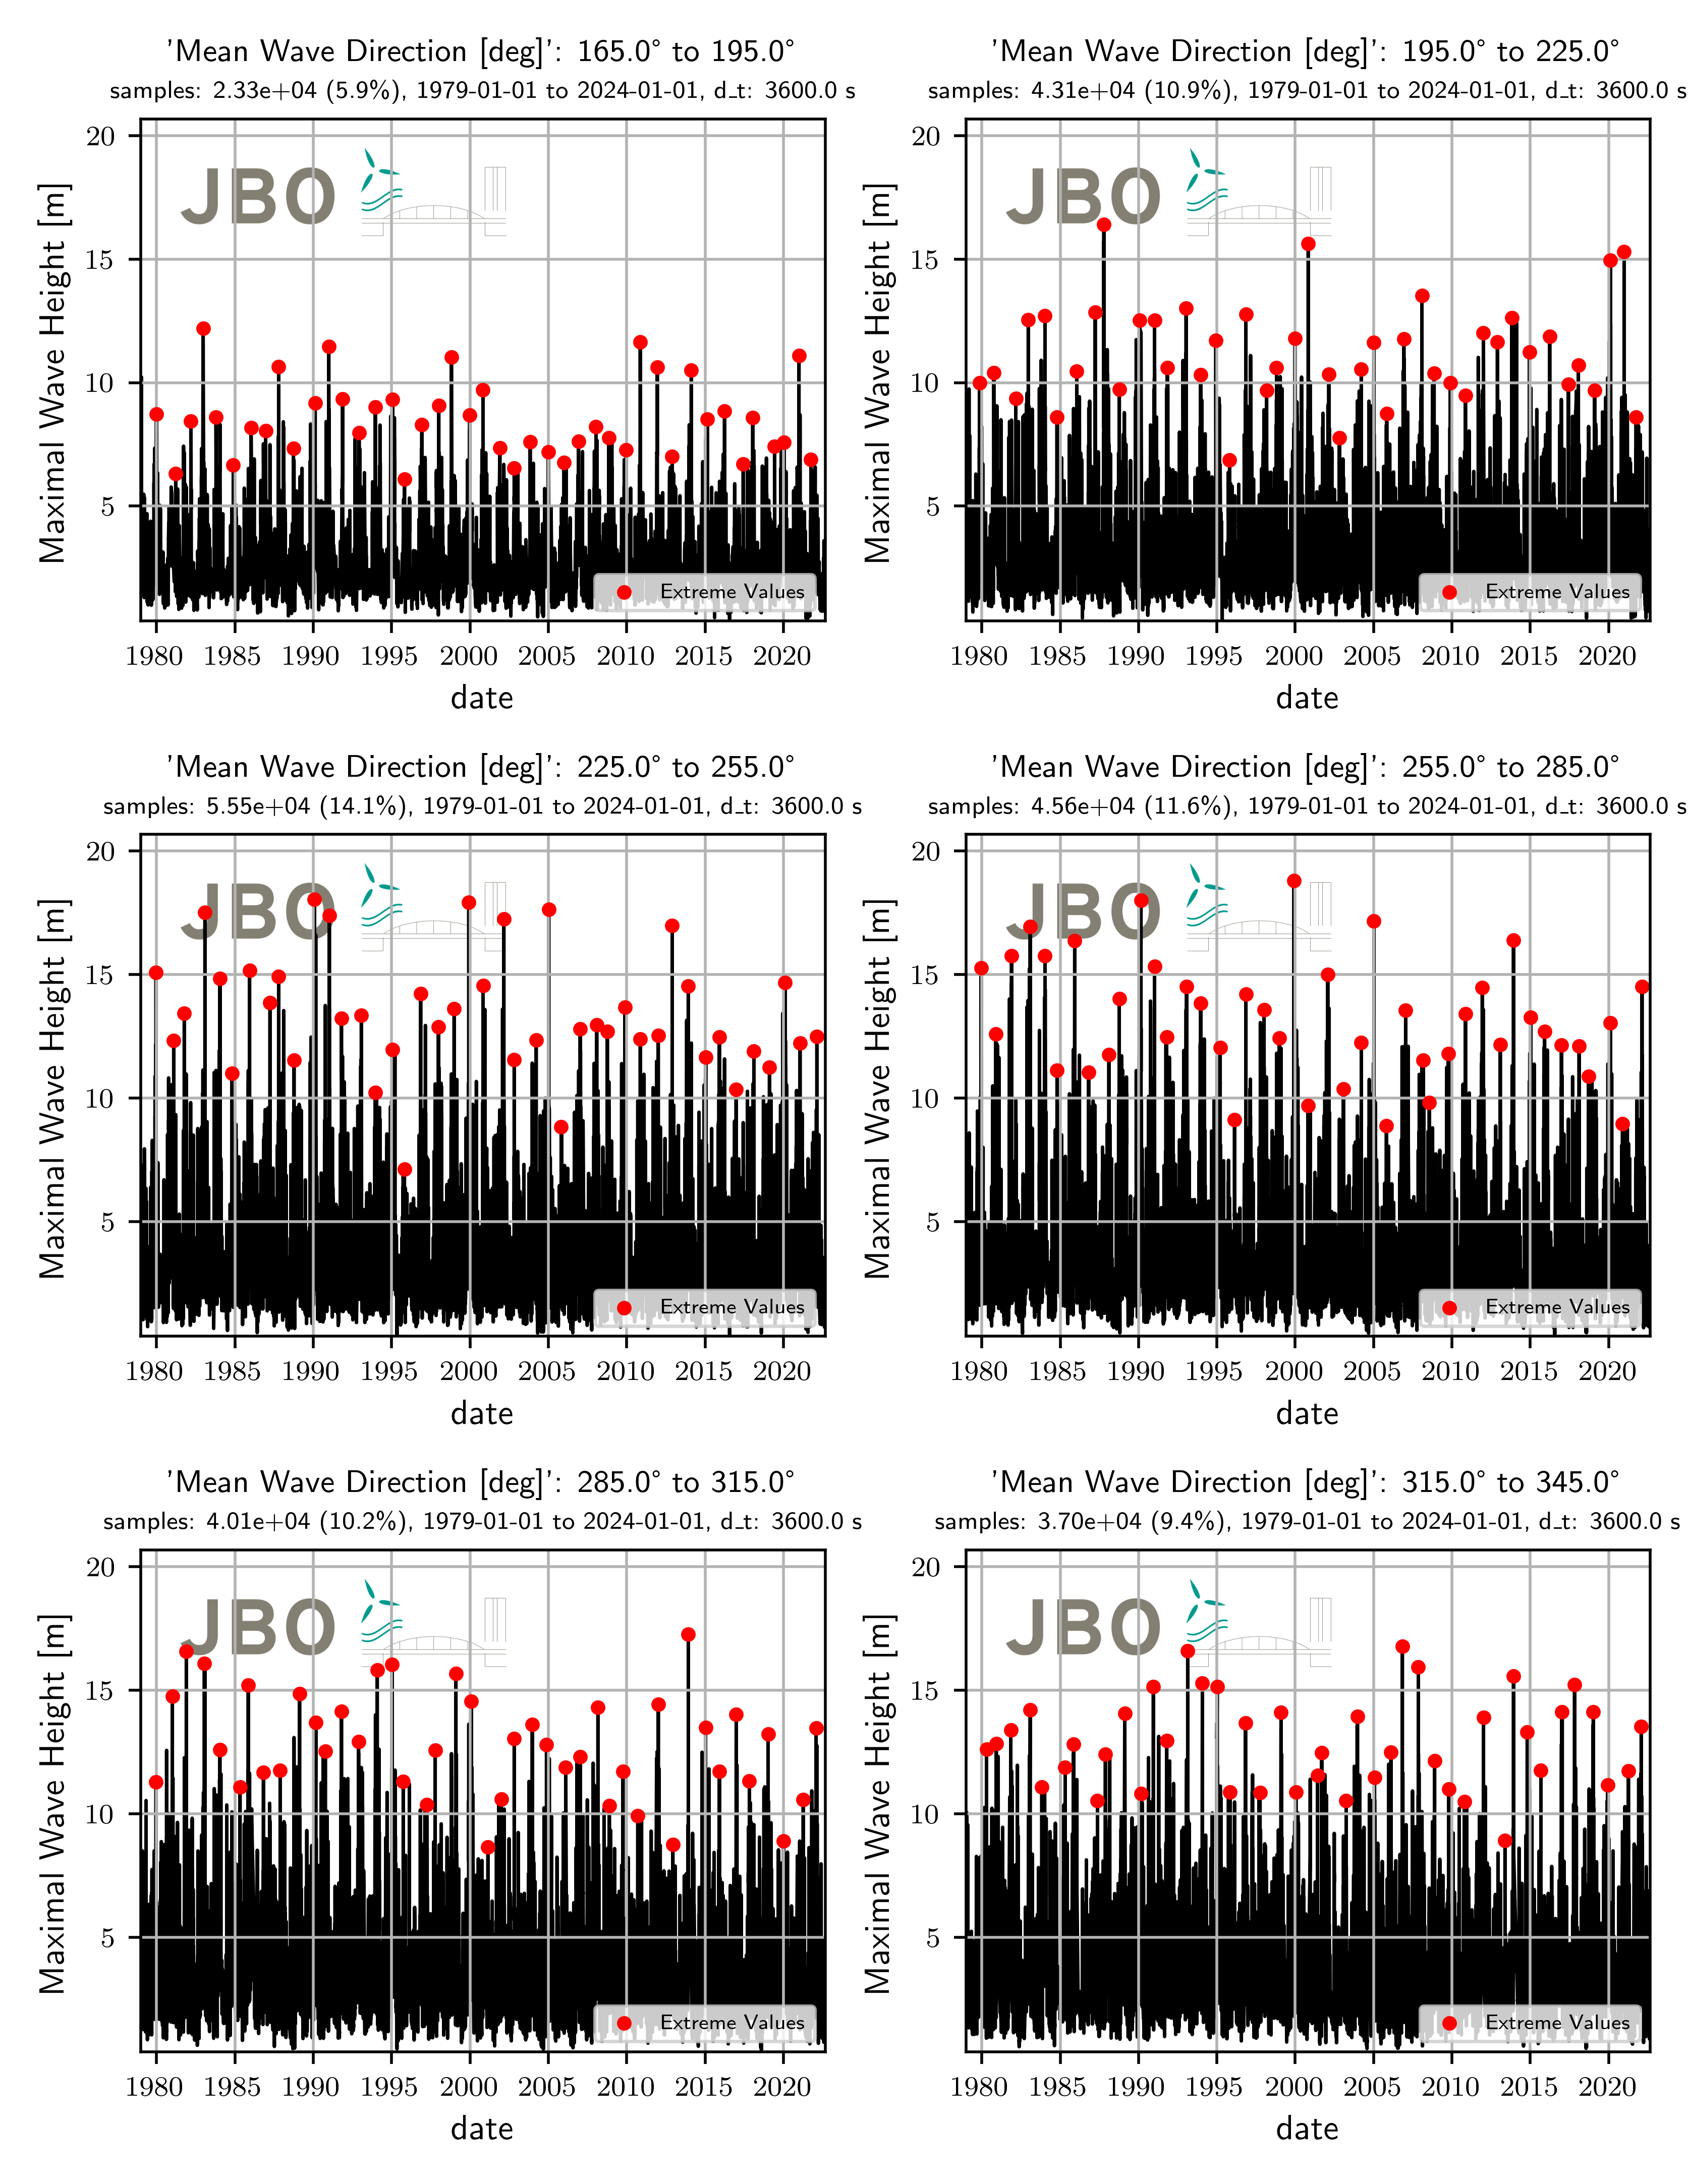
\includegraphics[width=1.0\textwidth]{C:/Users/aaron.lange/Desktop/Projekte/Hindcast_Tool/HindTool/example_output/Extreme_Timeseries_WaveHeight_page_2.png} 
 \caption{ Extreme-Timeseries-WaveHeight-page-2 } 
 \label{fig: Extreme_Timeseries_WaveHeight_page_2 } 
\end{figure}
\begin{figure}[H] 
 \centering 
 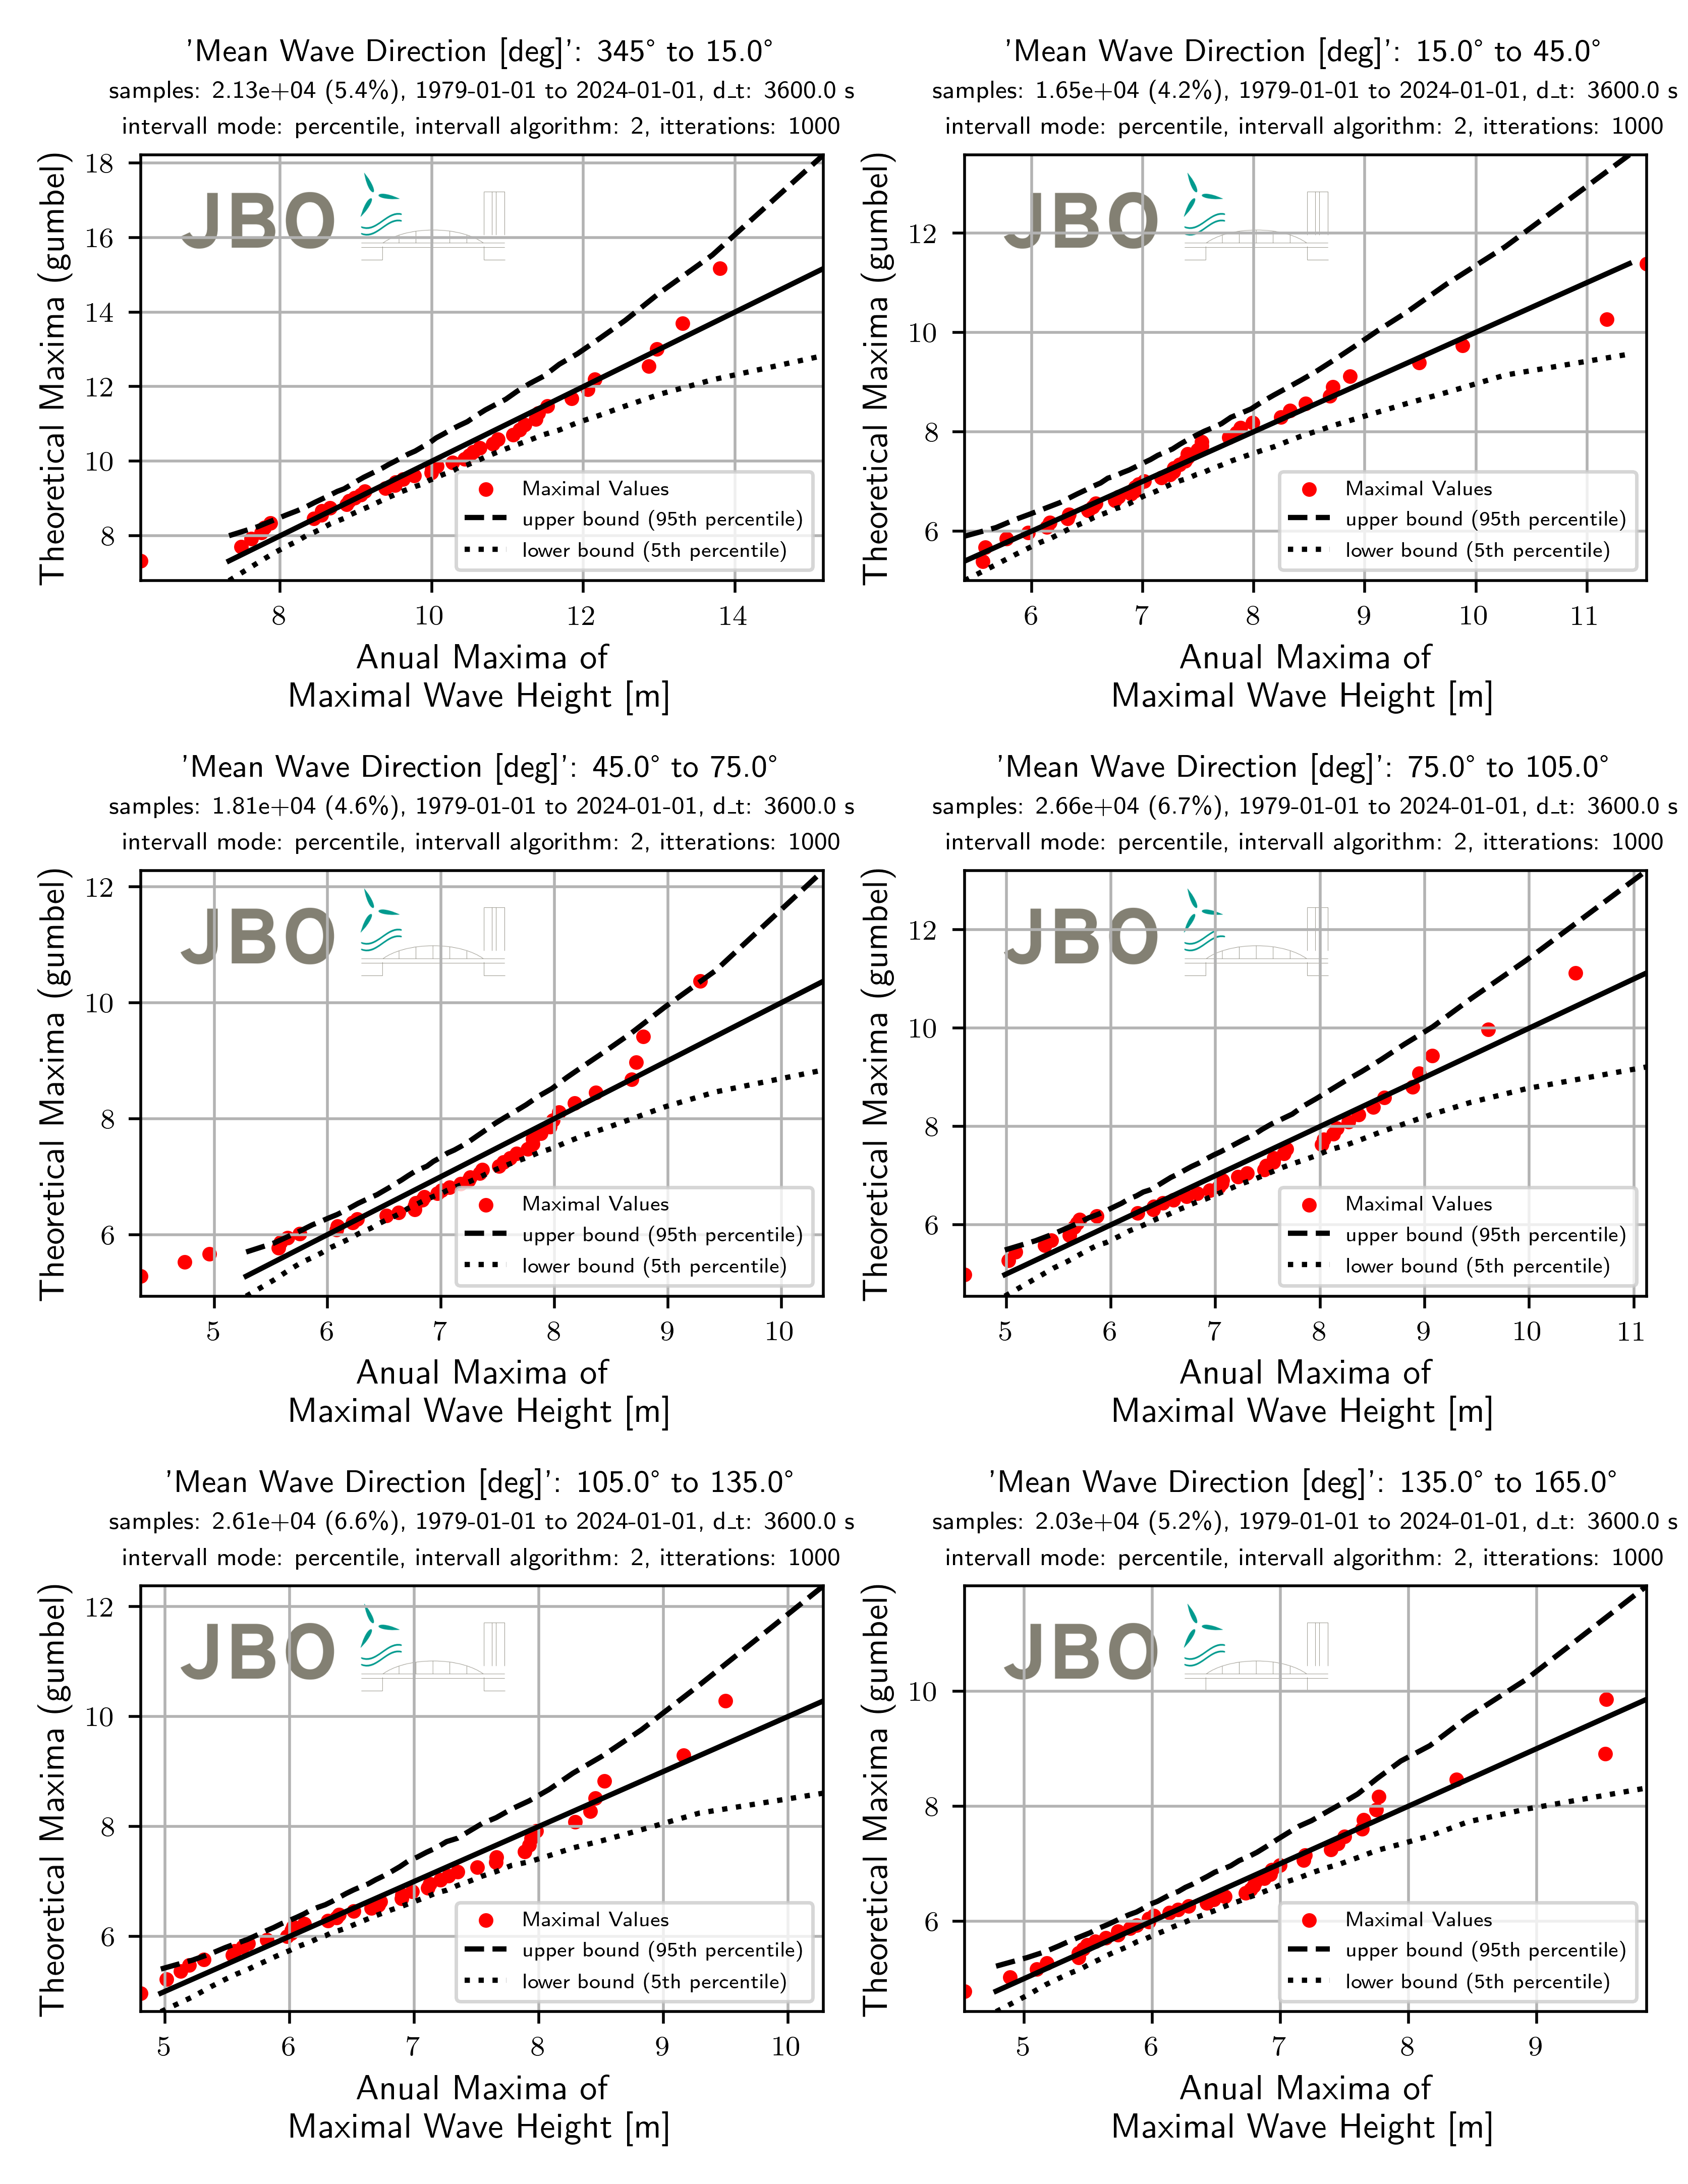
\includegraphics[width=1.0\textwidth]{C:/Users/aaron.lange/Desktop/Projekte/Hindcast_Tool/HindTool/example_output/Extreme_qq_WaveHeight_page_1.png} 
 \caption{ Extreme-qq-WaveHeight-page-1 } 
 \label{fig: Extreme_qq_WaveHeight_page_1 } 
\end{figure}
\begin{figure}[H] 
 \centering 
 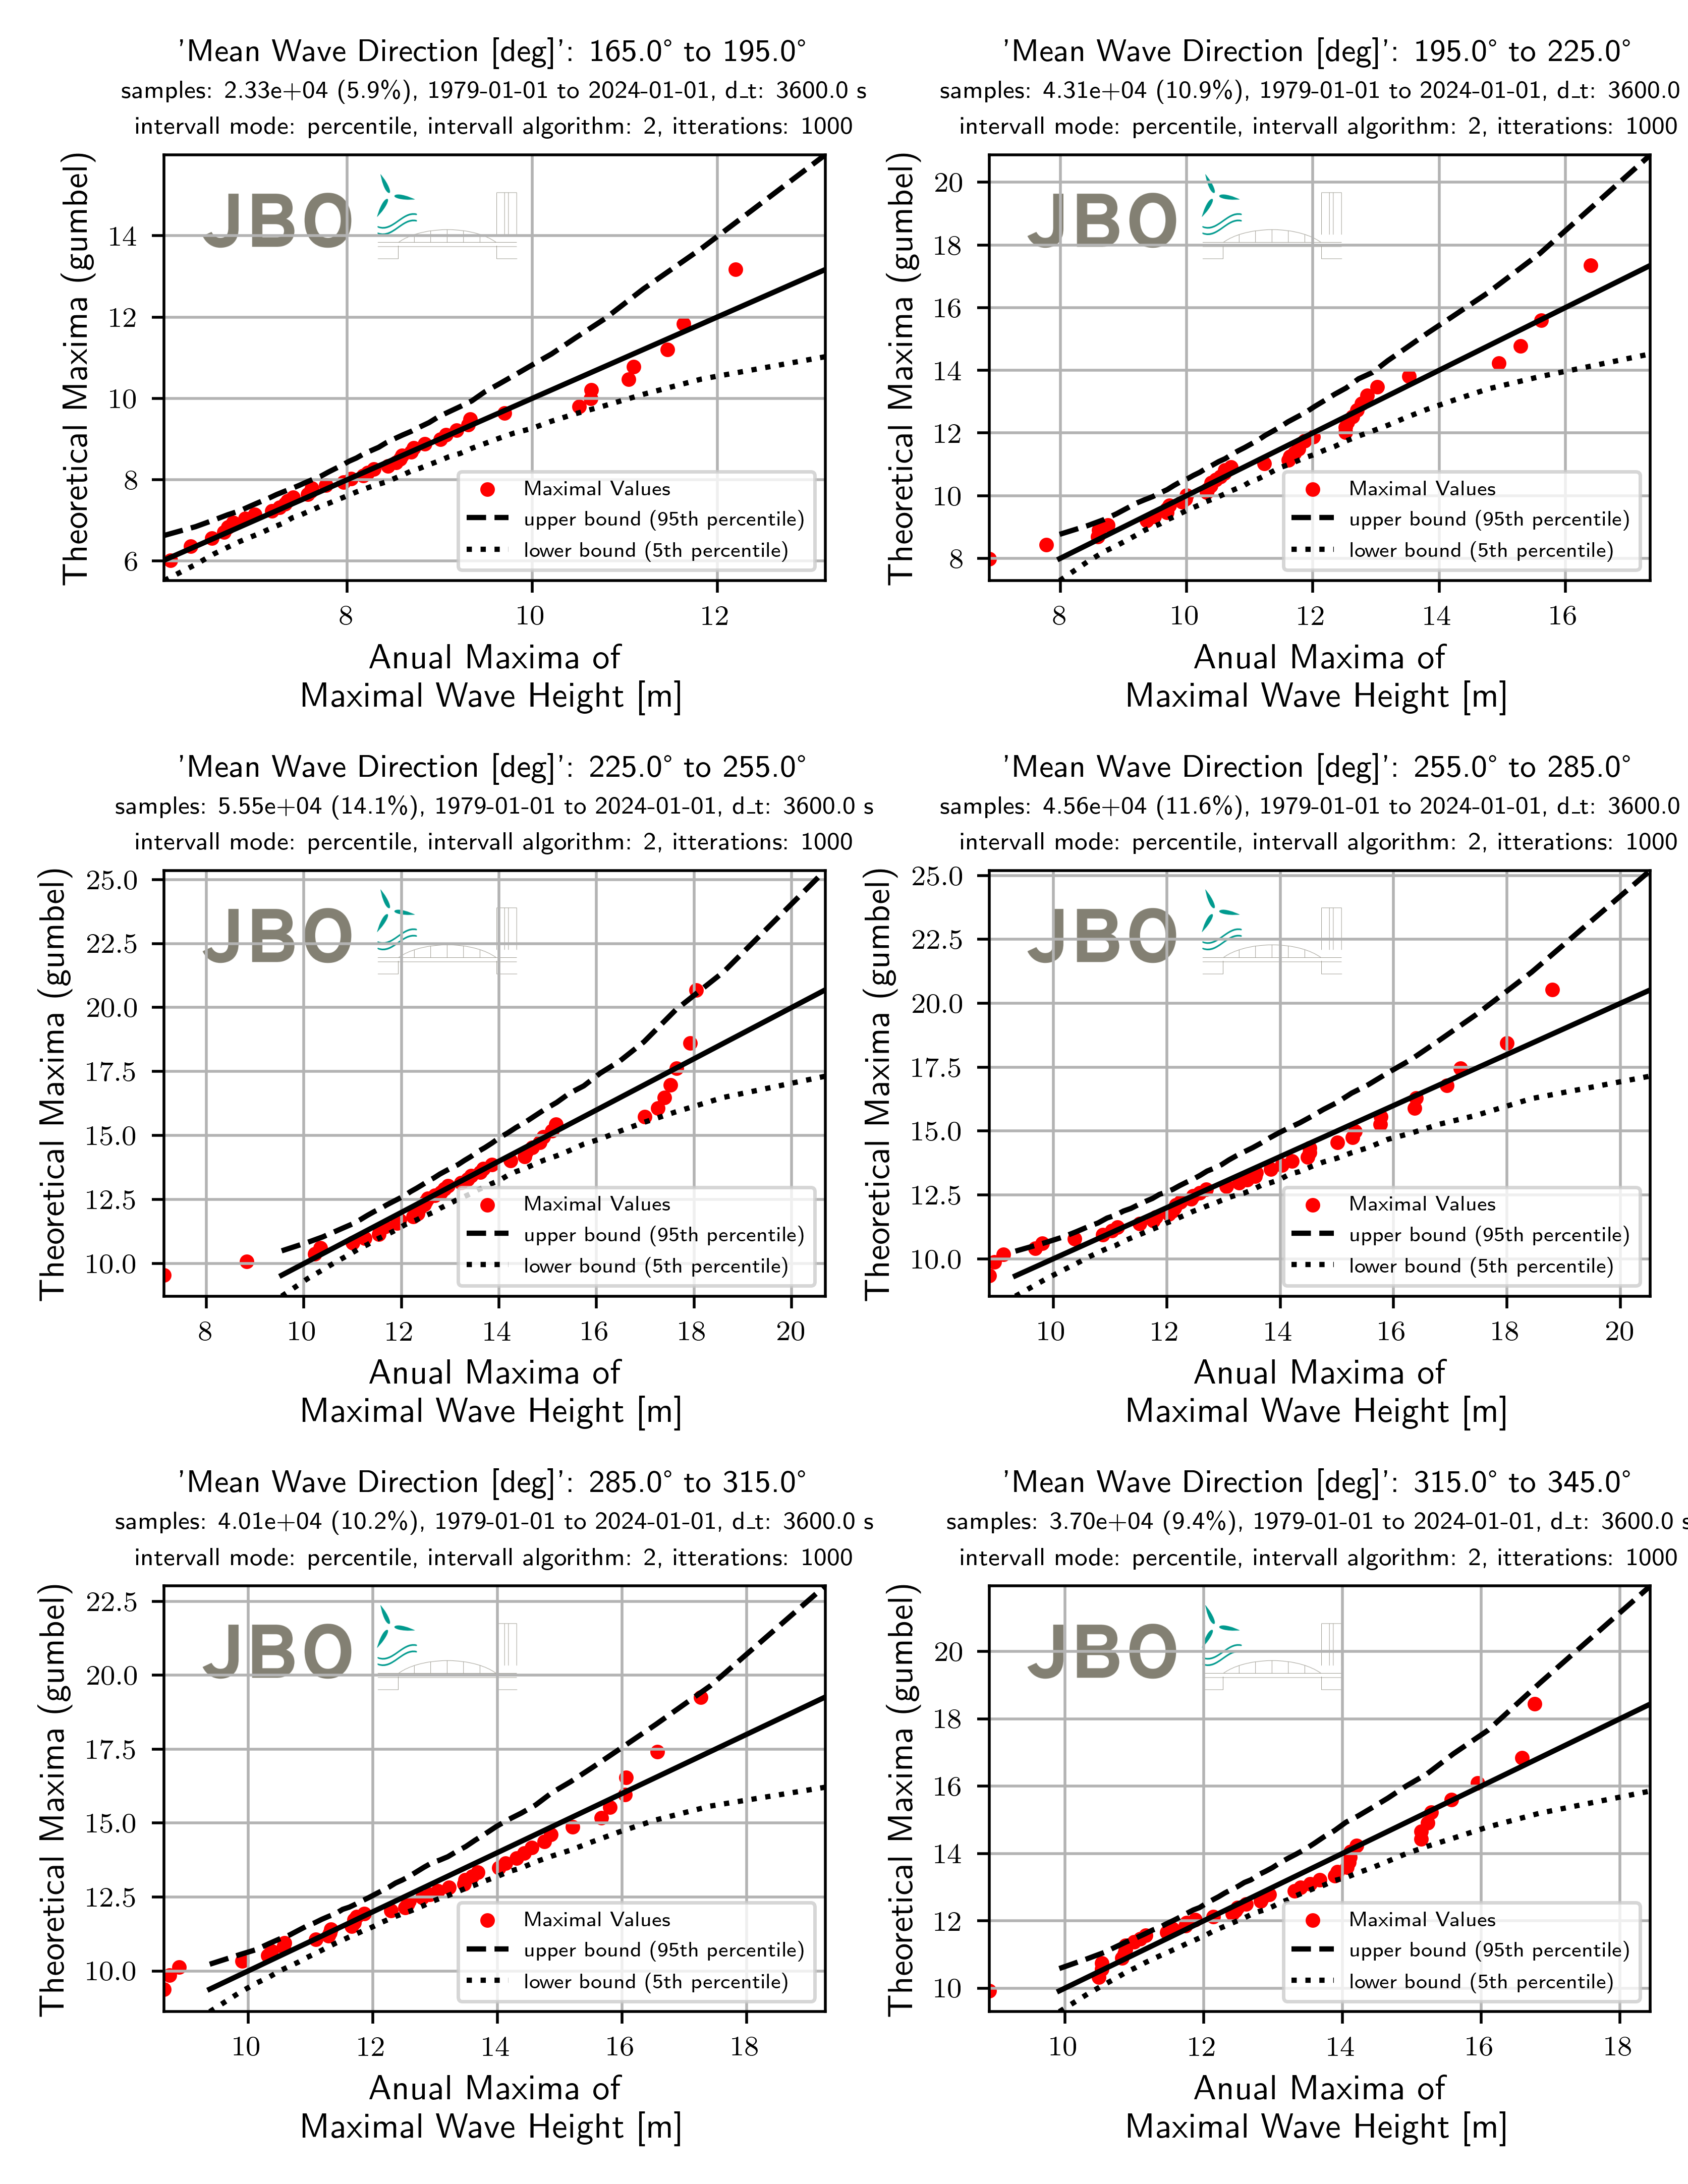
\includegraphics[width=1.0\textwidth]{C:/Users/aaron.lange/Desktop/Projekte/Hindcast_Tool/HindTool/example_output/Extreme_qq_WaveHeight_page_2.png} 
 \caption{ Extreme-qq-WaveHeight-page-2 } 
 \label{fig: Extreme_qq_WaveHeight_page_2 } 
\end{figure}
\begin{figure}[H] 
 \centering 
 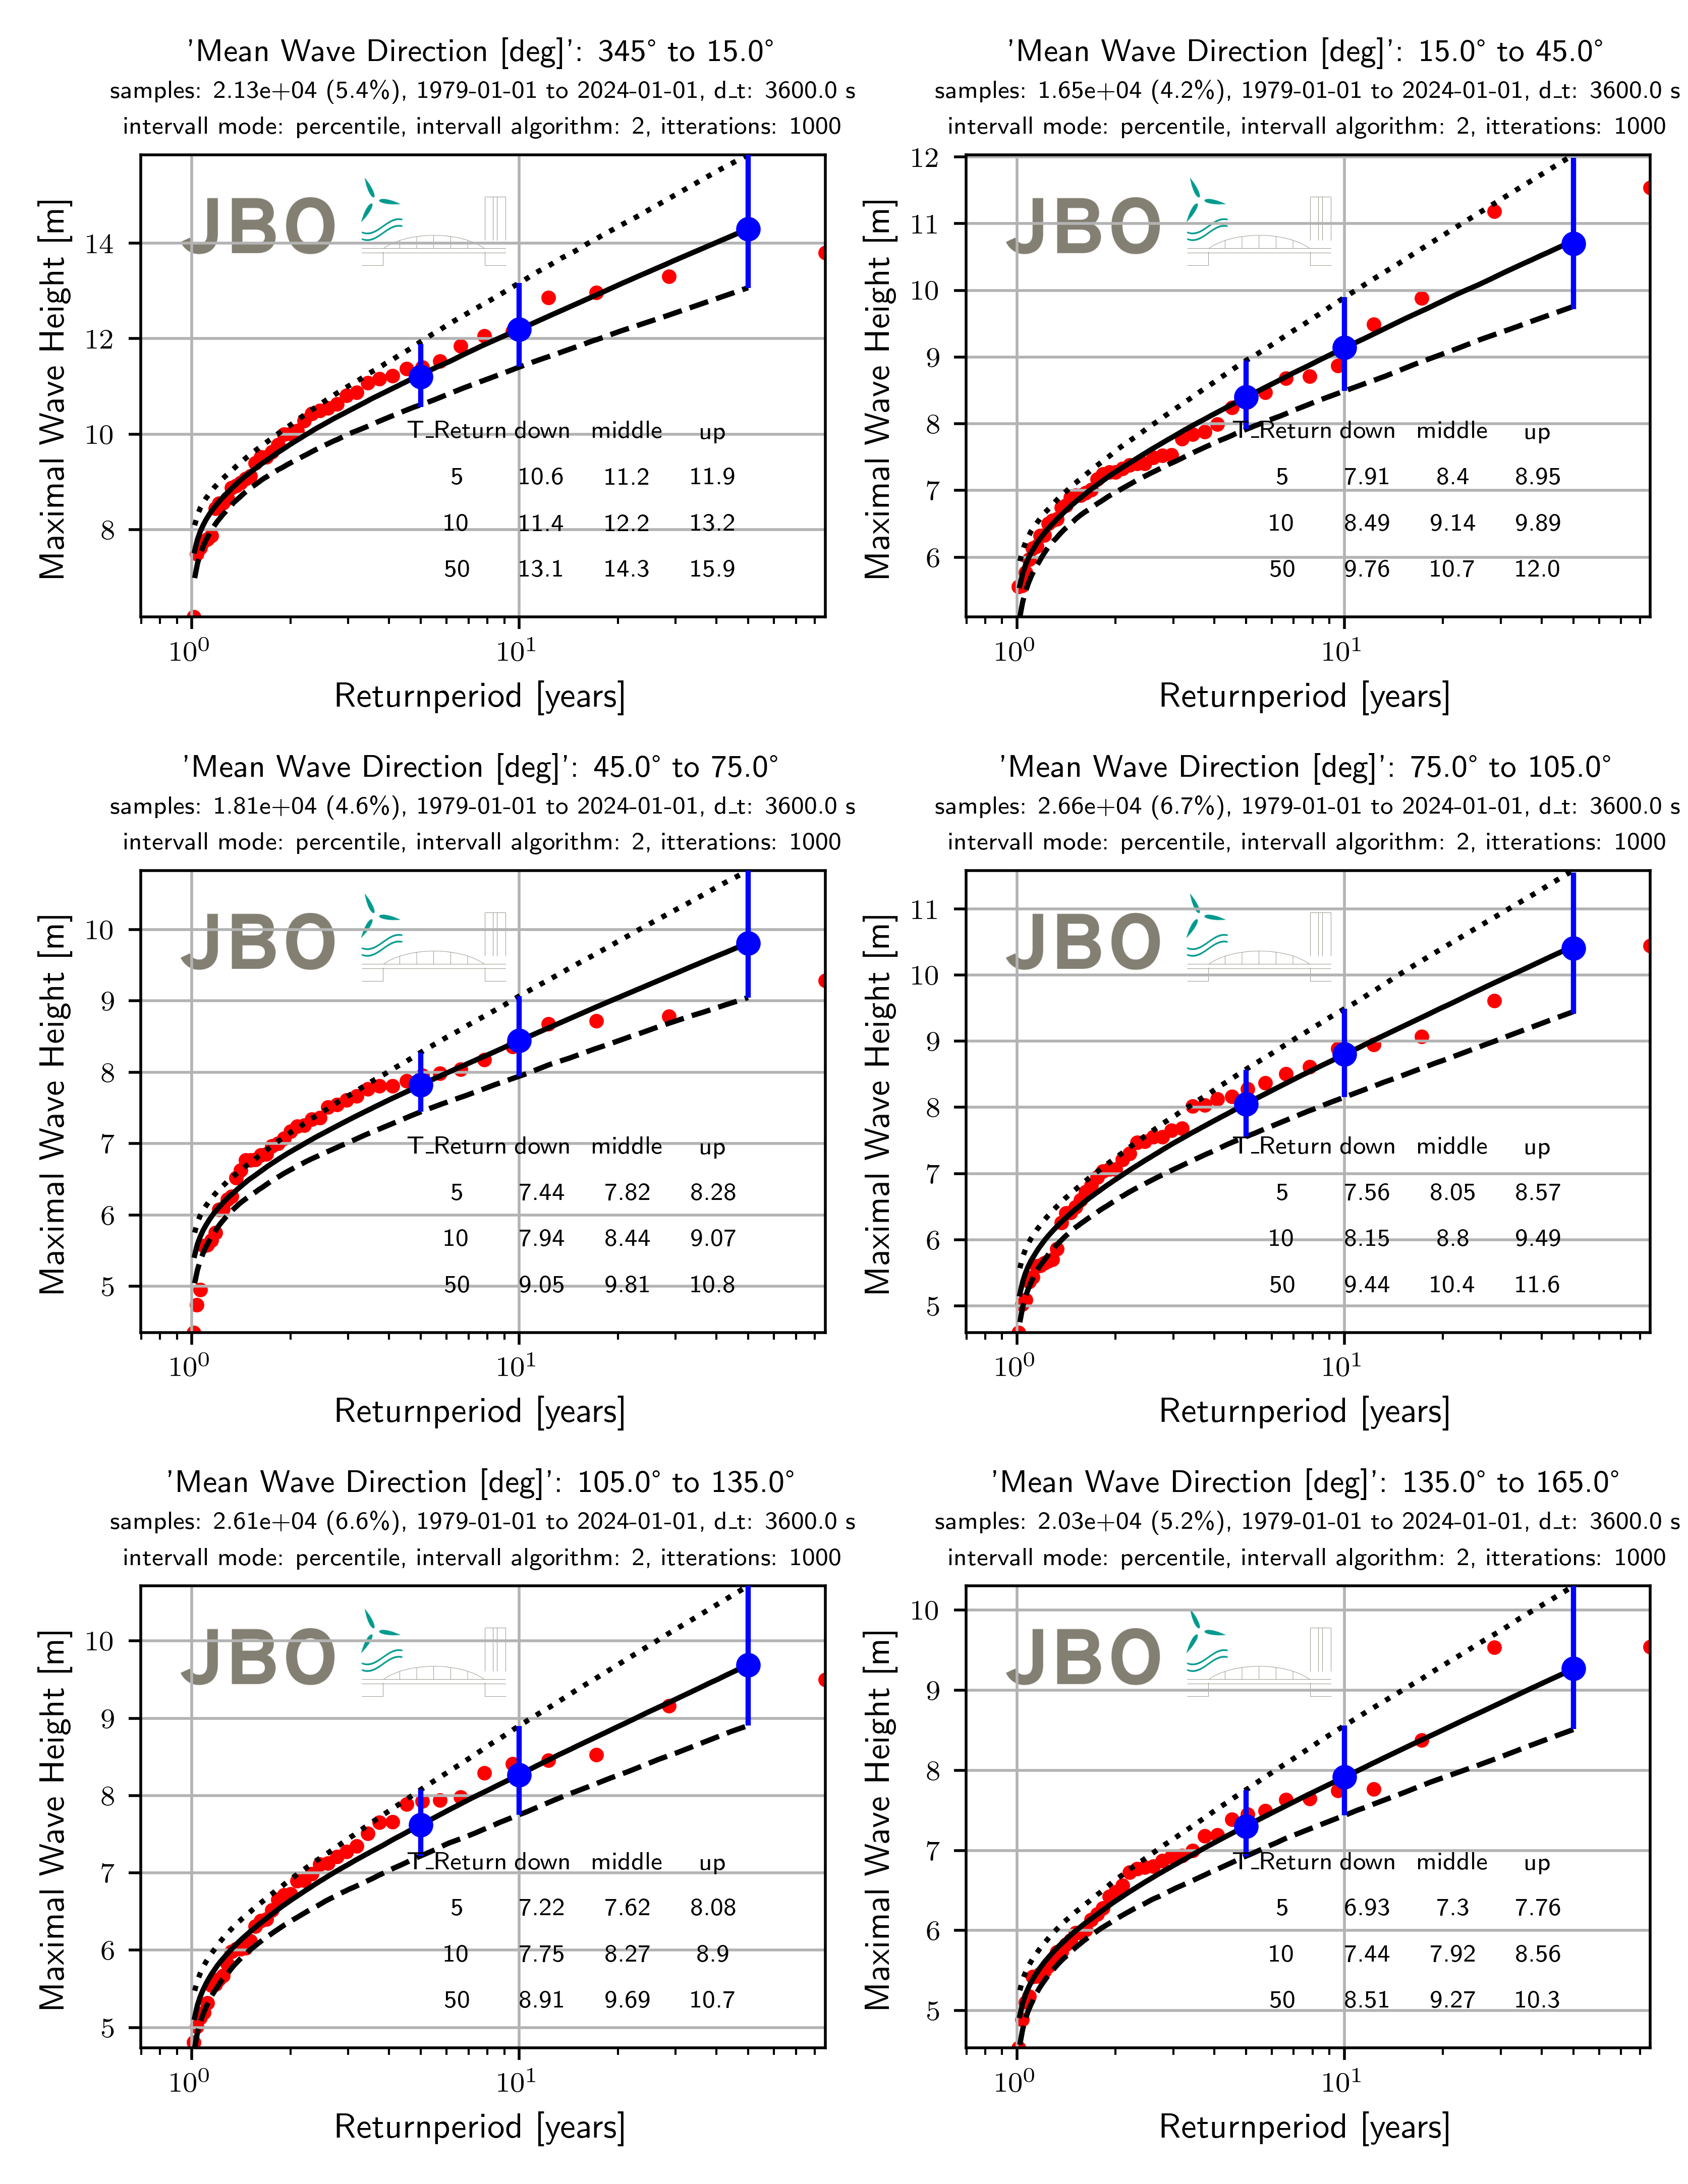
\includegraphics[width=1.0\textwidth]{C:/Users/aaron.lange/Desktop/Projekte/Hindcast_Tool/HindTool/example_output/Extreme_T_return_WaveHeight_page_1.png} 
 \caption{ Extreme-T-return-WaveHeight-page-1 } 
 \label{fig: Extreme_T_return_WaveHeight_page_1 } 
\end{figure}
\begin{figure}[H] 
 \centering 
 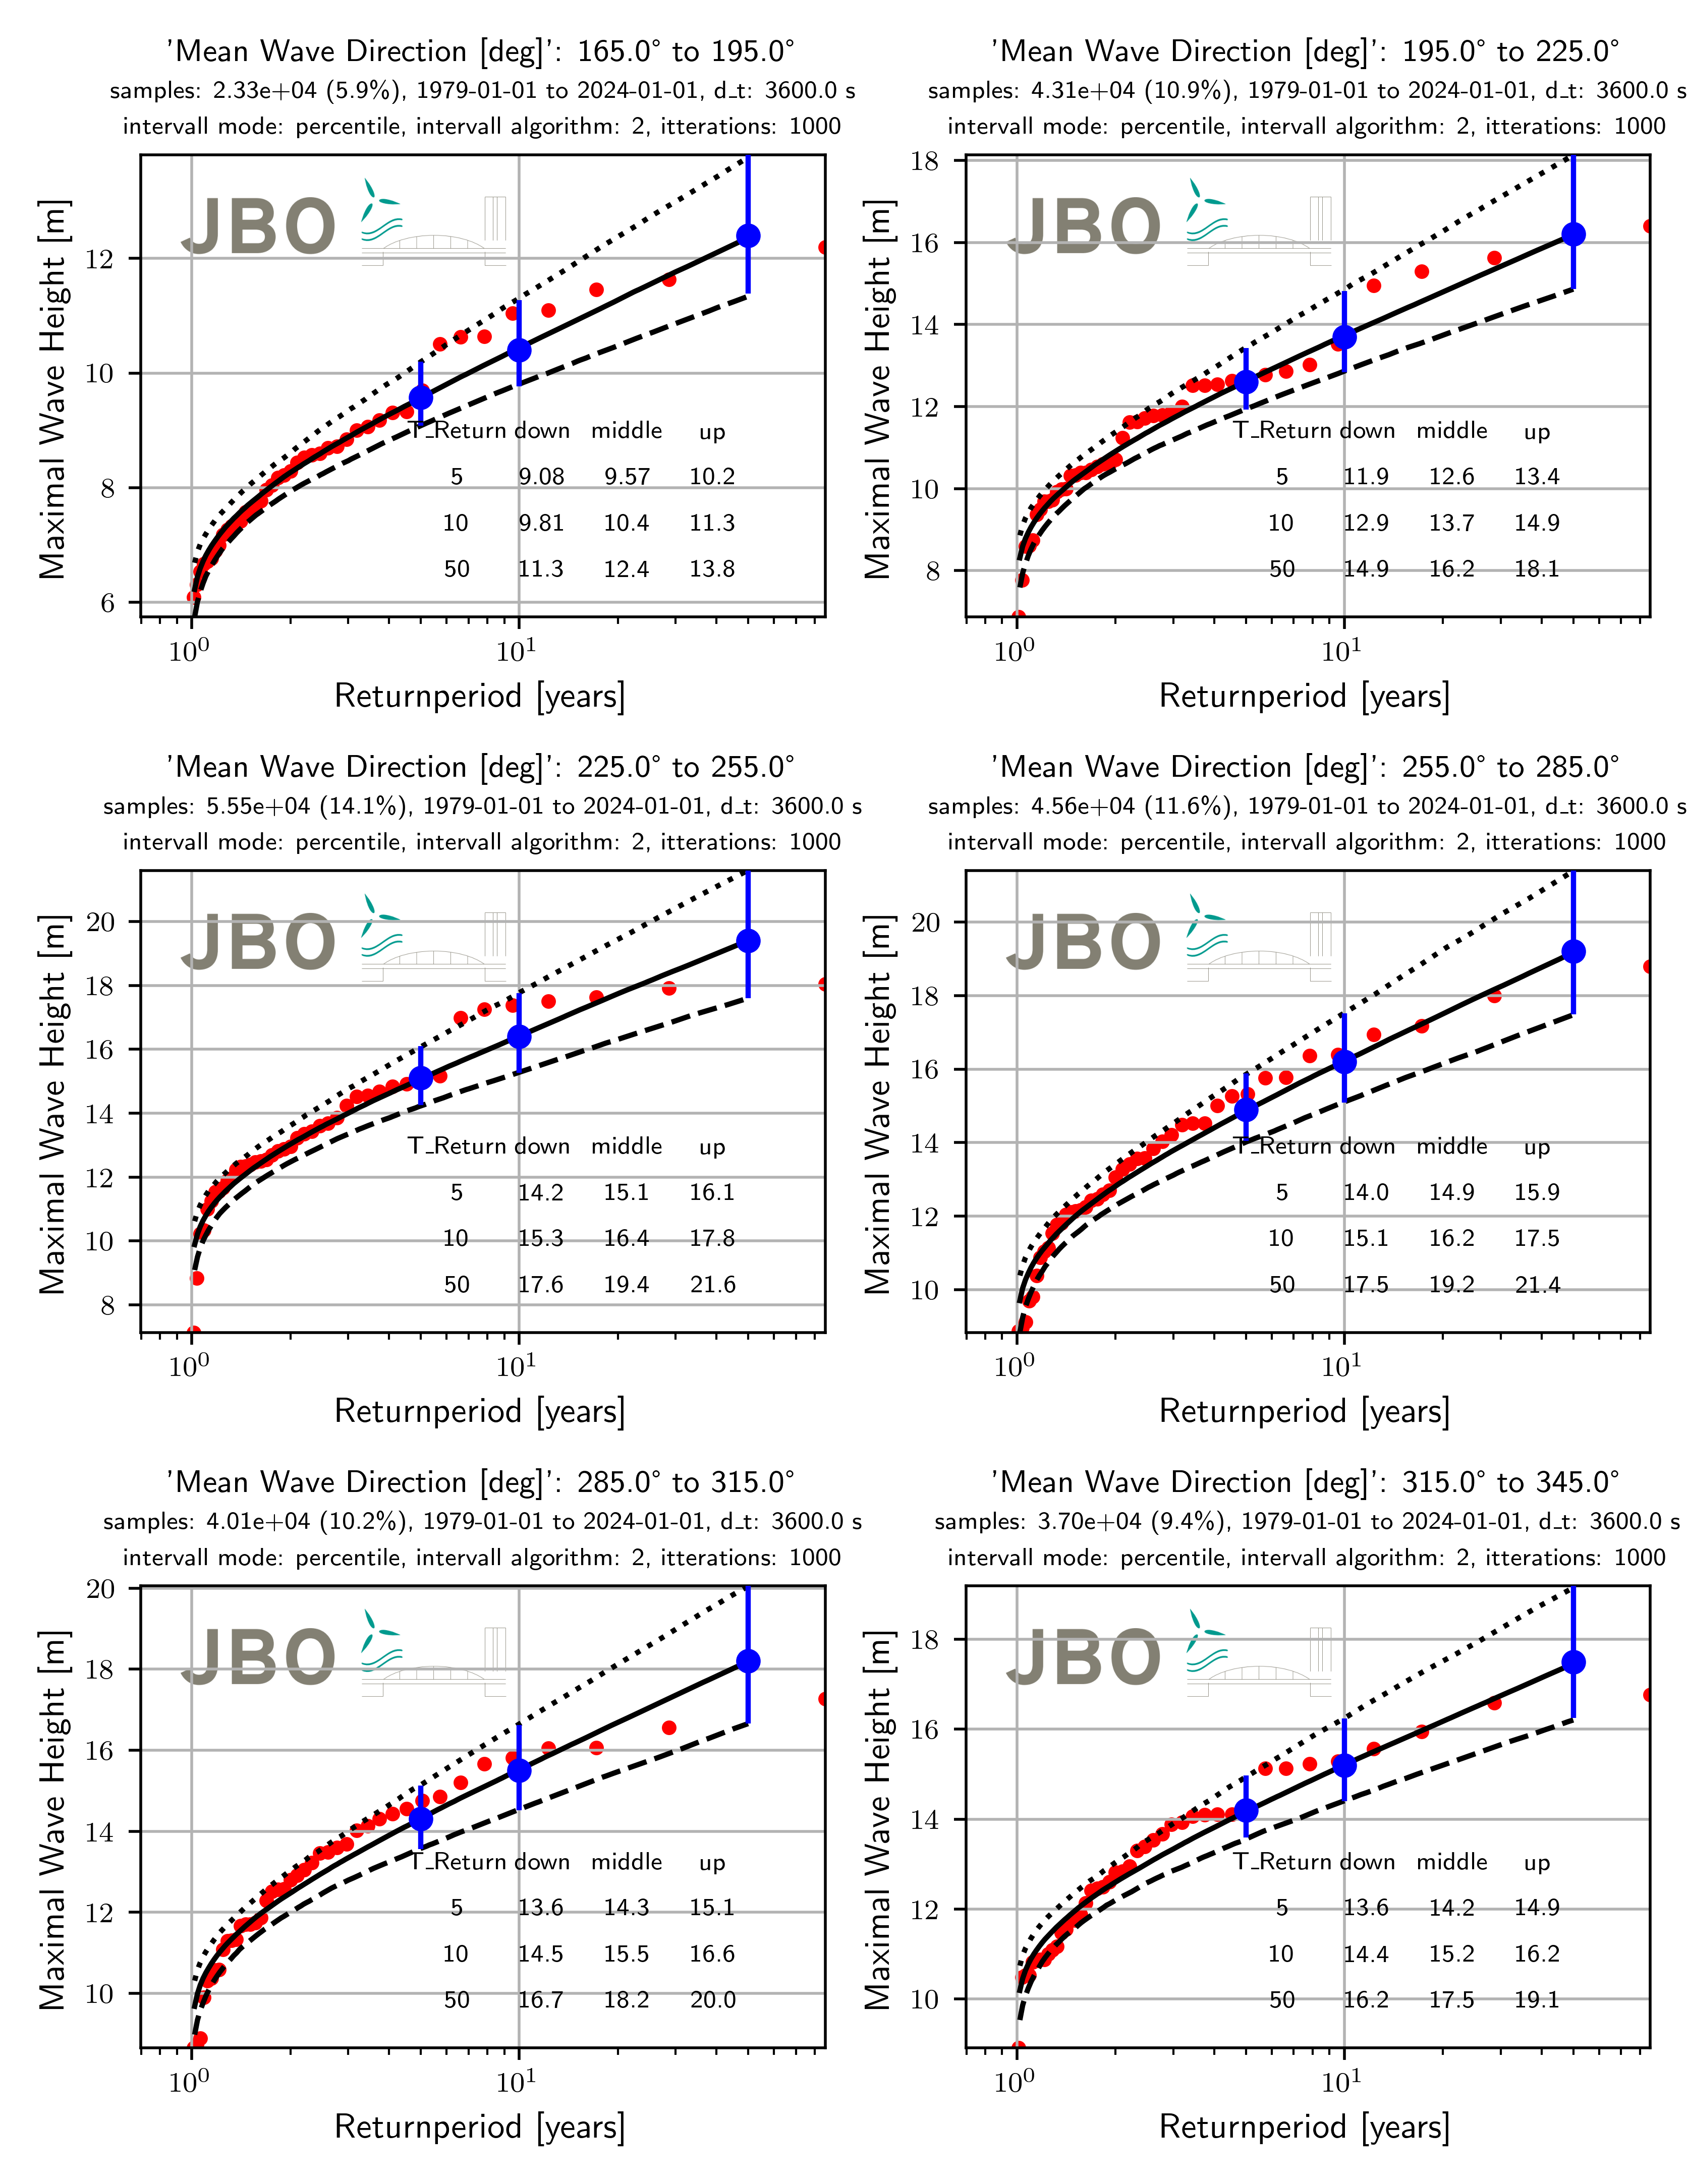
\includegraphics[width=1.0\textwidth]{C:/Users/aaron.lange/Desktop/Projekte/Hindcast_Tool/HindTool/example_output/Extreme_T_return_WaveHeight_page_2.png} 
 \caption{ Extreme-T-return-WaveHeight-page-2 } 
 \label{fig: Extreme_T_return_WaveHeight_page_2 } 
\end{figure}

